\documentclass[]{article}
\usepackage{lmodern}
\usepackage{amssymb,amsmath}
\usepackage{ifxetex,ifluatex}
\usepackage{fixltx2e} % provides \textsubscript
\ifnum 0\ifxetex 1\fi\ifluatex 1\fi=0 % if pdftex
  \usepackage[T1]{fontenc}
  \usepackage[utf8]{inputenc}
\else % if luatex or xelatex
  \ifxetex
    \usepackage{mathspec}
    \usepackage{xltxtra,xunicode}
  \else
    \usepackage{fontspec}
  \fi
  \defaultfontfeatures{Mapping=tex-text,Scale=MatchLowercase}
  \newcommand{\euro}{€}
\fi
% use upquote if available, for straight quotes in verbatim environments
\IfFileExists{upquote.sty}{\usepackage{upquote}}{}
% use microtype if available
\IfFileExists{microtype.sty}{%
\usepackage{microtype}
\UseMicrotypeSet[protrusion]{basicmath} % disable protrusion for tt fonts
}{}
\ifxetex
  \usepackage[setpagesize=false, % page size defined by xetex
              unicode=false, % unicode breaks when used with xetex
              xetex]{hyperref}
\else
  \usepackage[unicode=true]{hyperref}
\fi
\usepackage[usenames,dvipsnames]{color}
\hypersetup{breaklinks=true,
            bookmarks=true,
            pdfauthor={Ivo Hofacker, Dominik Steininger, Sven Findeiß, and many more\\},
            pdftitle={ViennaRNA Tutorial},
            colorlinks=true,
            citecolor=blue,
            urlcolor=blue,
            linkcolor=magenta,
            pdfborder={0 0 0}}
\urlstyle{same}  % don't use monospace font for urls
\usepackage{longtable,booktabs}
\usepackage{graphicx,grffile}
\makeatletter
\def\maxwidth{\ifdim\Gin@nat@width>\linewidth\linewidth\else\Gin@nat@width\fi}
\def\maxheight{\ifdim\Gin@nat@height>\textheight\textheight\else\Gin@nat@height\fi}
\makeatother
% Scale images if necessary, so that they will not overflow the page
% margins by default, and it is still possible to overwrite the defaults
% using explicit options in \includegraphics[width, height, ...]{}
\setkeys{Gin}{width=\maxwidth,height=\maxheight,keepaspectratio}
\setlength{\parindent}{0pt}
\setlength{\parskip}{6pt plus 2pt minus 1pt}
\setlength{\emergencystretch}{3em}  % prevent overfull lines
\providecommand{\tightlist}{%
  \setlength{\itemsep}{0pt}\setlength{\parskip}{0pt}}
\setcounter{secnumdepth}{0}

\title{ViennaRNA Tutorial}
\date{2017-08-02 20:50:00}
\author{Ivo Hofacker, Dominik Steininger, Sven Findeiß, and many more}
% Redefines (sub)paragraphs to behave more like sections
\ifx\paragraph\undefined\else
\let\oldparagraph\paragraph
\renewcommand{\paragraph}[1]{\oldparagraph{#1}\mbox{}}
\fi
\ifx\subparagraph\undefined\else
\let\oldsubparagraph\subparagraph
\renewcommand{\subparagraph}[1]{\oldsubparagraph{#1}\mbox{}}
\fi

\begin{document}
\maketitle


\includegraphics{Figs/unilogo_small.png}

\href{http://www.tbi.univie.ac.at/}{Theoretical Biochemistry Group}
\href{https://www.tbi.univie.ac.at/index.html}{
\includegraphics{Figs/tbilogo.png}}

\href{https://www.tbi.univie.ac.at/software}{Software}
\href{https://www.tbi.univie.ac.at/RNA/index.html}{ViennaRNA}
\href{https://www.tbi.univie.ac.at/RNA/tutorial/tutorial.html}{Tutorial}

\section{A short Tutorial on RNA Bioinformatics\\
The ViennaRNA Package and related Programs}
\url{http://www.tbi.univie.ac.at/RNA/}\\

This tutorial aims to give a basic introduction to using the programs
in the ViennaRNA Package.

\subsection{Get started}\label{get-started}

\subsubsection{What's in the \texttt{ViennaRNA\ Package}}{What's in the ViennaRNA Package}\label{whats-in-the-viennarna-package}

The core of the \texttt{ViennaRNA\ Package} is formed by a collection
of routines for the prediction and comparison of RNA secondary
structures.  These routines can be accessed through stand-alone
programs, such as \texttt{RNAfold}, \texttt{RNAdistance} etc., which
should be sufficient for most users. For those who wish to develop
their own programs a library which can be linked to your own code is
provided.

\paragraph{Which programs are available?}\\
\begin{itemize}
\item \texttt{RNA2Dfold} Compute coarse grained energy landscape of representative
sample structures \\
\item \texttt{RNAaliduplex} Predict conserved RNA-RNA interactions
between two alignments\\
\item \texttt{RNAalifold} Calculate secondary structures for a set of aligned RNA sequences\\
\item \texttt{RNAcofold} Calculate secondary structures of two RNAs with dimerization\\
\item \texttt{RNAdistance} Calculate distances between RNA secondary structures \\
\item \texttt{RNAduplex} Compute the structure upon hybridization of two RNA strands\\
\item \texttt{RNAeval} Evaluate free energy of RNA sequences with given secondary structure\\
\item \texttt{RNAfold} Calculate minimum free energy secondary structures and partition function of RNAs\\
\item \texttt{RNAheat} Calculate the specific heat (melting curve) of an RNA sequence
\item \texttt{RNAinverse} Find RNA sequences with given secondary structure (sequence design)
\item \texttt{RNALalifold} Calculate locally stable secondary structures for a set of aligned RNAs\\
\item \texttt{RNALfold} Calculate locally stable secondary structures of long RNAs\\
\item \texttt{RNApaln} RNA alignment based on sequence base pairing propensities\\
\item \texttt{RNApdist} Calculate distances between thermodynamic RNA secondary structures ensembles\\
\item \texttt{RNAparconv} Convert energy parameter files from ViennaRNA 1.8 to 2 format\\
\item \texttt{RNAPKplex} Predict RNA secondary structures including pseudoknots\\
\item \texttt{RNAplex} Find targets of a query RNA\\
\item \texttt{RNAplfold} Calculate average pair probabilities for locally stable secondary structures\\
\item \texttt{RNAplot} Draw and markup RNA secondary structures in PostScript, SVG, or GML\\
\item \texttt{RNApvmin} Find a vector of perturbation energies which may further be used to constrain folding\\
\item \texttt{RNAsnoop} Find targets of a query H/ACA snoRNA\\
\item \texttt{RNAsubopt} Calculate suboptimal secondary structures of RNAs\\
\item \texttt{RNAup} Calculate the thermodynamics of RNA-RNA interactions\\
\item \texttt{Kinfold} simulates the stochastic folding kinetics of RNA sequences into secondary structures \\
\item \texttt{RNAforester} compare RNA secondary structures via forest alignment\\
\end{itemize}

\subsubsection{The Input File Format}{The Input File Format}\label{the-input-file-format}

RNA sequences come in a variety of formats. The sequence format used
throughout the ViennaRNA Package is very simple. A sequence file
contains one or more sequences. Each sequence must appear as a single
line in the file without embedded white spaces. A sequence may be
preceded by a special line starting with the `\texttt{\textgreater{}}'
character followed by a sequence name. This name will be used by the
programs in the \texttt{ViennaRNA\ Package} as basename for the
PostScript output files for this sequence. Note that this is almost the
\texttt{fasta} sequence format, except that no line-breaks are allowed
within a sequence while the header line is optional. Following programs
provide full fasta support:
\texttt{RNAfold,\ RNAsubopt,\ RNAcofold,\ RNAKplex,\ RNALfold,\ RNAplfold,\ RNAeval,\ RNAplot,\ RNAheat}

\subsection{Structure Prediction on single Sequences}{Structure Prediction on single Sequences}\label{structure-prediction-on-single-sequences}

\subsubsection{The Program \texttt{RNAfold}}{The Program RNAfold}\label{the-program-rnafold}

Our first task will be to do a structure prediction using
\texttt{RNAfold}. This should get you familiar with the input and output
format as well as the graphical output produced. \texttt{RNAfold} reads
RNA sequences from \emph{stdin}, calculates their minimum free energy
(\texttt{MFE}) structure, prints the \texttt{MFE} structure in
dot-bracket notation and its free energy to \emph{stdout}. If the
\texttt{-p} option is set it also computes the partition function, the
base pairing probability matrix and additionally prints the free energy
of the thermodynamic ensemble, the frequency of the \texttt{MFE}
structure in the ensemble and the ensemble diversity to \emph{stdout}.
Another useful option is the \texttt{-\/-MEA} option, which also shows
the maximum expected accuracy, but remember that this also needs more
CPU time than without \texttt{-\/-MEA}.

\textbf{MFE structure of a single sequence}\\
1. Use a text editor (emacs, vi, nano, gedit) to prepare an input file by
pasting the text below and save it under the name \texttt{test.seq} in
your \texttt{Data} folder.

\hyperdef{}{verbatim-18}{\label{verbatim-18}}
\begin{verbatim}
``` {.commands}
> test
CUACGGCGCGGCGCCCUUGGCGA
```

</div>
\end{verbatim}

\begin{enumerate}
\def\labelenumi{\arabic{enumi}.}
\setcounter{enumi}{1}
\tightlist
\item
  Compute the best (MFE) structure for this sequence

  \hyperdef{}{verbatim-19}{\label{verbatim-19}}
\begin{verbatim}
$ RNAfold < test.seq
CUACGGCGCGGCGCCCUUGGCGA
...........((((...)))). ( -5.00)
\end{verbatim}
\end{enumerate}

The last line of the text output contains the predicted MFE structure as
dot-bracket notation and its free energy in \texttt{kcal/mol}. A dot in
the dot-bracket notation represents an unpaired position, while a base
pair (i, j) is represented by a pair of matching parentheses at position
i and j.

\texttt{RNAfold} created a file named \texttt{test\_ss.eps}. The filename
is taken from the fasta header; if there's no header the output is
simply called \texttt{rna.eps}.\\
Let's take a look at the output file with \texttt{gv}, a
PostScript{{[}\^{}2\^{}{]}(https://www.tbi.univie.ac.at/RNA/tutorial/tutorial3.html\#fn2x0)}\hyperdef{}{x1-19003f2}{\label{x1-19003f2}}{}
viewer. The \& at the end starts the program in the background.

\hyperdef{}{verbatim-20}{\label{verbatim-20}}
\begin{verbatim}
$ gv test_ss.ps &
\end{verbatim}

Compare the dot-bracket notation to the PostScript drawing shown in the
file \texttt{test\_ss.eps}.

The calculation above does not tell us whether the predicted structure
is the only possibility or not, so let's look at the equilibrium
ensemble instead.

\textbf{Predicting equilibrium pair probabilities}\\
1. Run \texttt{RNAfold\ -p\ -\/-MEA} to compute the partition function
and pair probabilities as well as the maximum expected accurarcy. 2.
Look at the generated PostScript files \texttt{test\_ss.eps} and
\texttt{test\_dp.eps}

\hyperdef{}{verbatim-21}{\label{verbatim-21}}
\begin{verbatim}
``` {.commands}
$ RNAfold -p --MEA < test.seq
  CUACGGCGCGGCGCCCUUGGCGA
  ...........((((...)))). ( -5.00)
  ....{,{{...||||...)}}}. [ -5.72]
  ....................... {  0.00 d=4.66}
  ......((...))((...))... {  2.90 MEA=14.79}
  frequency of mfe structure in ensemble 0.311796; ensemble diversity 6.36
```

</div>
\end{verbatim}

Here the last four lines are new compared to the text output without the
\texttt{-p\ -\/-MEA} options. The partition function is a rough measure
for the well-definedness of the \texttt{MFE} structure. The third line
shows a condensed representation of the pair probabilities of each
nucleotide, similar to the dot-bracket notation, followed by the
ensemble free energy (-kT ln(Z)) in \texttt{kcal/mol}. The next two
lines represent the centroid structure with its free energy, its
distance to the ensemble and the MEA. The last line shows the frequency
of the MFE structure in the ensemble of secondary structures and the
diversity of the ensemble.

''.'' denotes bases that are essentially unpaired, '','' weakly paired,
''\(|\)''strongly paired without preference, ''\{\},()'' weakly
(\textgreater{}33\%) upstream (downstream) paired or strongly (\textgreater{}66\%)
up-/downstream paired bases, respectively.\\
 Note that the MFE structure is adopted only with 31\% probability, also
the diversity is very high for such a short sequence.\\
 For rotating the secondary structure plot there is a usefull tool
called \texttt{rotate\_ss.pl} included in the ViennaRNA Package. Just
read the \texttt{perldoc} for this tool to know how to handle the
rotation and use the information to get your secondary structure in a
vertical position.

\begin{verbatim}
$ perldoc rotate_ss.pl
\end{verbatim}

\textbf{Secondary Structure plot and Dot plot}\\
 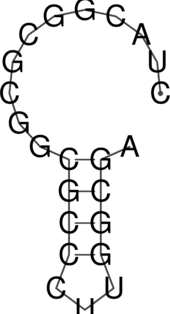
\includegraphics{Figs/test_ss.png}

\includegraphics{Figs/test_dp.png}\\
The ``dot plot'' in \texttt{test\_dp.eps} shows the pair probabilities
within the equilibrium ensemble as \(n \times n\) matrix, and is an
excellent way to visualize structural alternatives. A square at row
\(i\) and column \(j\) indicates a base pair. The area of a square in
the upper right half of the matrix is proportional to the probability of
the base pair \(\left( {i,j} \right)\) within the equilibrium ensemble.
The lower left half shows all pairs belonging to the \texttt{MFE}
structure. While the MFE consists of a single helix, several different
helices are visualized in the pair probabilities.\\
 Next, let's use the \texttt{relplot} utility to visualize which parts
of a predicted MFE are well-defined and thus more reliable. Also let's
use a real example for a change and produce yet another representation
of the predicted structure, the \emph{mountain plot}.

\textbf{Mountain and Reliability plot}\\
 Fold the 5S rRNA sequence and visualize the structure. (The
\texttt{5S.seq} is shipped with the tutorial)

\hyperdef{}{verbatim-23}{\label{verbatim-23}}
\begin{verbatim}
$ RNAfold -p < 5S.seq
$ mountain.pl 5S_dp.ps | xmgrace -pipe
$ relplot.pl 5S_ss.ps 5S_dp.ps > 5S_rss.ps
\end{verbatim}

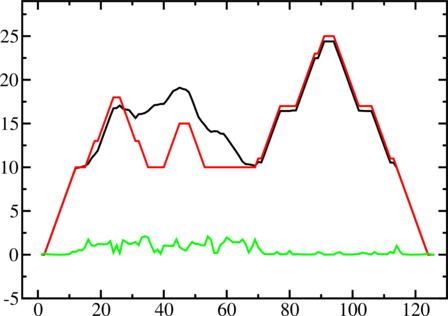
\includegraphics{Figs/5S_mt.png}
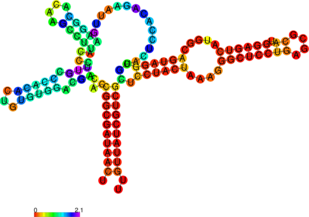
\includegraphics{Figs/5S_rot.png}

A mountain plot is especially useful for long sequences where
conventional structure drawings become terribly cluttered. It is a
xy-diagram plotting the number of base pairs enclosing a sequence
position \emph{versus} the position. The \texttt{Perl} script
\texttt{mountain.pl} transforms a dot plot into the mountain plot
coordinates which can be visualized with any xy-plotting program, e.g.
\texttt{xmgrace}.

The resulting plot shows three curves, two mountain plots derived from
the \texttt{MFE} structure (red) and the pairing probabilities (black)
and a positional entropy curve (green). Well-defined regions are
identified by low entropy. By superimposing several mountain plots
structures can easily be compared.\\
 The perl script \texttt{relplot.pl} adds reliability information to a
RNA secondary structure plot in the form of color annotation. The script
computes a well-definedness measure we call ``positional entropy''
(\(S\left( i \right) = - \sum p_{ij}\log\left( p_{ij} \right)\) for
those who want to know the details) and encodes it as color hue, ranging
from red (low entropy, well-defined) via green to blue and violet (high
entropy, ill-defined). In the example above two helices of the 5S RNA are
well-defined (red) and indeed predicted correctly, the left arm is not
quite correct and disordered.\\
For the figure above we had to rotate and mirror the structure plot, e.g.

\hyperdef{}{verbatim-24}{\label{verbatim-24}}
\begin{verbatim}
$ rotate_ss.pl -a 180 -m 5S_rss.ps > 5S_rot.ps
\end{verbatim}

You can manually add annotation to structure drawings using the RNAplot
program (for information see the \texttt{man} page). Here's a somewhat
complicated example:

\hyperdef{}{verbatim-25}{\label{verbatim-25}}
\begin{verbatim}
$ RNAfold < 5S.seq > 5S.fold
$ RNAplot --pre "76 107 82 102 GREEN BFmark 44 49 0.8 0.8 0.8 Fomark \
   1 15 8 RED omark 80 cmark 80 -0.23 -1.2 (pos80) Label 90 95 BLUE Fomark" < 5S.fold
$ gv 5S_ss.ps
\end{verbatim}

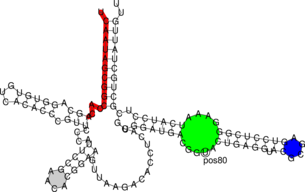
\includegraphics{Figs/5S_ss.png}\\

\texttt{RNAplot} is a very useful tool to color plots. The
\texttt{-\/-pre} tag adds PostScript code to color distinct regions of
your molecule. There are some predefined statements with different options
for annotations listed below:

\texttt{i\ cmark} draws circle around base i \texttt{i\ j\ c\ gmark}
draw basepair i,j with c counter examples in grey
\texttt{i\ j\ lw\ rgb\ omark} stroke segment i\ldots{}j with linewidth
lw and color (rgb) \texttt{i\ j\ rgb\ Fomark} fill segment i\ldots{}j
with color (rgb) \texttt{i\ j\ k\ l\ rgb\ BFmark} fill block between
pairs i,j and k,l with color (rgb) \texttt{i\ dx\ dy\ (text)\ Label}
adds a textlabel with an offset dx and dy relative to base i

Predefined color options are \texttt{BLACK,\ RED,\ GREEN,\ BLUE,\ WHITE}
but you can also replace the value to some standard RGB code (e.g.~0 5 8
for lightblue).\\
 To see what exactly the alternative structures of our sequence are, we
need to predict \emph{suboptimal} structures.

\textbf{SHAPE directed RNA folding}\\
In order to further improve the quality of secondary structure
predictions, mapping experiments like SHAPE (selective 2'-hydroxyl
acylation analyzed by primer extension) can be used to exerimentally
determine the pairing status for each nucleotide. In addition to
thermodynamic based secondary structure predictions, RNAfold supports
the incorporation of this additional experimental data as soft
constraints.

If you want to use SHAPE data to guide the folding process, please make
sure that your experimental data is present in a text file, where each
line stores three white space separated columns containing the position,
the abbreviation and the normalized SHAPE reactivity for a certain
nucleotide.

\hyperdef{}{verbatim-26}{\label{verbatim-26}}
\begin{verbatim}
    1 G 0.134
    2 C 0.044
    3 C 0.057
    4 G 0.114
    5 U 0.094
      ...
      ...
      ...
    71 C 0.035
    72 G 0.909
    73 C 0.224
    74 C 0.529
    75 A 1.475
\end{verbatim}

The second column, which holds the nucleotide abbreviation, is optional.
If it is present, the data will be used to perform a cross check against
the provided input sequence. Missing SHAPE reactivities for certain
positions can be indicated by omitting the reactivity column or the
whole line. Negative reactivities will be treated as missing. Once the
SHAPE file is ready, it can be used to constrain folding:

\begin{verbatim}
$ RNAfold --shape=rna.shape --shapeMethod=D < rna.seq
\end{verbatim}

\subsubsection{The Program \texttt{RNApvmin}}{The Program RNApvmin}\label{the-program-rnapvmin}

The program \texttt{RNApvmin} reads a RNA sequence from \emph{stdin} and
uses an iterative minimization process to calculate a perturbation
vector that minimizes the discripancies between predicted pairing
probabilites and observed pairing probabilities (deduced from given
shape reactivities). The experimental SHAPE data has to be present in
the file format described above. The application will write the
calculated vector of perturbation energies to \emph{stdout}, while the
progress of the minimization process is written to \emph{stderr}. The
resulting perturbation vector can be interpreted directly and gives
usefull insights into the discrepancies between thermodynamic prediction
and experimentally determined pairing status. In addition the
perturbation energies can be used to constrain folding with
\texttt{RNAfold}:

\begin{verbatim}
$ RNApvmin rna.shape < rna.seq >vector.csv
$ RNAfold --shape=vector.csv --shapeMethod=W < rna.seq
\end{verbatim}

The perturbation vector file uses the same file format as the SHAPE data
file. Instead of SHAPE reactivities the raw perturbation energies will be
storred in the last column. Since the energy model is only adjusted when
necessary, the calculated perturbation energies may be used for the
interpretation of the secondary structure prediction, since they
indicate which positions require major energy model adjustments in order
to yield a prediction result close to the experimental data. High
perturbation energies for just a few nucleotides may indicate the
occurrence of features, which are not explicitly handled by the energy
model, such as posttranscriptional modifications and intermolecular
interactions.

\subsubsection{The Program \texttt{RNAsubopt}}{The Program RNAsubopt}\label{the-program-rnasubopt}

\texttt{RNAsubopt} calculates all suboptimal secondary structures within
a given energy range above the \texttt{MFE} structure. Be careful, the
number of structures returned grows exponentially with both sequence
length and energy range.

\textbf{Suboptimal folding}\\
- Generate all suboptimal structures within a certain energy range from
the \texttt{MFE} specified by the \texttt{-e} option.

\begin{verbatim}
``` {.commands}
$ RNAsubopt -e 1 -s < test.seq
CUACGGCGCGGCGCCCUUGGCGA   -500    100
...........((((...)))).  -5.00
....((((...))))........  -4.80
(((.((((...))))..)))...  -4.20
...((.((.((...)).)).)).  -4.10
```
\end{verbatim}

The text output shows an energy sorted list (option \texttt{-s}) of all
secondary structures within 1~kcal/mol of the \texttt{MFE} structure.
Our sequence actually has a ground state structure (-5.70) and three
structures within 1~kcal/mol range.

\texttt{MFE} folding alone gives no indication that there are actually a
number of plausible structures. Remember that \texttt{RNAsubopt} cannot
automatically plot structures, therefore you can use the tool
\texttt{RNAplot}. Note that you CANNOT simply pipe the output of
\texttt{RNAsubopt} to \texttt{RNAplot} using

\begin{verbatim}
$ RNAsubopt < test.seq | RNAplot
\end{verbatim}

You need to manually create a file for each structure you want to plot.
Here, for example we created a new file named suboptstructure.txt:

\begin{verbatim}
> suboptstructure-4.20
CUACGGCGCGGCGCCCUUGGCGA
(((.((((...))))..)))...
\end{verbatim}

The fasta header is optional, but useful (without it the outputfile will
be named rna.ps). The next two lines contain the sequence and the
suboptimal structure you want to plot; in this case we plotted the
structure with the folding energy of -4.20. Then plot it with

\begin{verbatim}
$ RNAplot < suboptstructure.txt
\end{verbatim}

Note that the number of suboptimal structures grows exponentially with
sequence length and therefore this approach is only tractable for
sequences with less than 100 nt. To keep the number of suboptimal
structures manageable the option \texttt{-\/-noLP} can be used, forcing
\texttt{RNAsubopt} to produce only structures without isolated base
pairs. While \texttt{RNAsubopt} produces \emph{all} structures within an
energy range, \texttt{mfold} produces only a few, hopefully
representative, structures. Try folding the sequence on the mfold server
at\\
\url{http://mfold.rna.albany.edu/?q=mfold}.\\
 Sometimes you want to get information about unusual properties of the
Boltzmann ensemble (the sum of all RNA structures possible) for which no
specialized program exists. For example you want to know all fractions
of a bacterial mRNA in the Boltzmann ensemble where the Shine-Dalgarno
(SD) sequence is unpaired. If the SD sequence is concealed by secondary
structure the translation efficiency is reduced.

In such cases you can resort to drawing a representative sample of
structures from the Boltzmann ensemble by using the option \texttt{-p}.
Now you can simply count how many structures in the sample possess the
feature you are looking for. This number divided by the size of your
sample gives you the desired fraction.\\
 The following example calculates the fraction of structures in the
ensemble that have bases 6 to 8 unpaired.

\textbf{Sampling the Boltzmann Ensemble}\\
1. Draw a sample of size 10,000 from the Boltzmann ensemble 2. Calculate
the desired property by using a perl script

\begin{verbatim}
$ RNAsubopt -p 10000 < test.seq > tt
$ perl -nle '$h++ if substr($_,5,3) eq "...";
     END {print $h/$.}' tt
     0.391960803919608
\end{verbatim}

A far better way to calculate this property is to use
\texttt{RNAfold\ -p} to get the ensemble free energy, which is related
to the partition function via \(F = - RT\ln\left( Q \right)\), for the
unconstrained (\(F_{u}\)) and the constrained case (\(F_{c}\)), where
the three bases are not allowed to form base pairs (use option
\texttt{-C}), and evaluate
\(p_{c} = \exp\left( \left( {F_{u} - F_{c}} \right)\slash RT \right)\)
to get the desired probability.\\
 So let's do the calculation using \texttt{RNAfold}.

\begin{verbatim}
$RNAfold -p

Input string (upper or lower case); @ to quit
....,....1....,....2....,....3....,....4....,....5....,....6....,....7....,....8
CUACGGCGCGGCGCCCUUGGCGA
length = 23
CUACGGCGCGGCGCCCUUGGCGA
...........((((...)))).
 minimum free energy =  -5.00 kcal/mol
....{,{{...||||...)}}}.
 free energy of ensemble =  -5.72 kcal/mol
....................... {  0.00 d=4.66}
 frequency of mfe structure in ensemble 0.311796; ensemble diversity 6.36
\end{verbatim}

Now we have calculated the free ensemble energy of the ensemble over all
structures (F\_u), in the next step we have to calculate it for the
structures using a constraint(F\_c).\\
 Following notation has to be used for defining the constraint:

\begin{enumerate}
\def\labelenumi{\arabic{enumi}.}
\tightlist
\item
  \(|\) : paired with another base
\item
  . : no constraint at all
\item
  x : base must not pair
\item
  \(<\) : base i is paired with a base j¡i
\item
  \(>\) : base i is paired with a base j¿i
\item
  matching brackets ( ): base i pairs base j\\
\end{enumerate}

So our constraint should look like this:

\begin{verbatim}
  .....xxx...............
\end{verbatim}

Next call the application with following command and provide the
sequence and constraint we just created.

\begin{verbatim}
$ RNAfold -p -C
\end{verbatim}

The output should look like this

\begin{verbatim}
length = 23
CUACGGCGCGGCGCCCUUGGCGA
...........((((...)))).
 minimum free energy =  -5.00 kcal/mol
...........((((...)))).
 free energy of ensemble =  -5.14 kcal/mol
...........((((...)))). { -5.00 d=0.42}
 frequency of mfe structure in ensemble 0.792925; ensemble diversity 0.79
\end{verbatim}

Afterwards evaluate the desired probability according to the formula
given before e.g.~with a simple perl script.

\begin{verbatim}
$ perl -e 'print exp(-(5.72-5.14)/(0.00198*310.15))."\n"'
\end{verbatim}

You can see that there is a slight difference between the
\texttt{RNAsubopt} run with 10,000 samples and the \texttt{RNAfold} run
including all structures.

\subsection{RNA folding kinetics}{RNA folding kinetics}\label{rna-folding-kinetics}

RNA folding kinetics describes the dynamical process of how a RNA
molecule approaches to its unique folded biological active conformation
(often referred to as the native state) starting from an initial
ensemble of disordered conformations e.g.~the unfolded open chain. The
key for resolving the dynamical behavior of a folding RNA chain lies in
the understanding of the ways in which the molecule explores its
astronomically large free energy landscape, a rugged and complex
hyper-surface established by all the feasible base pairing patterns a
RNA sequence can form. The challenge is to understand how the interplay
of formation and break up of base pairing interactions along the RNA
chain can lead to an efficient search in the energy landscape which
reaches the native state of the molecule on a biologically meaningful
time scale.

\subsubsection{RNA2Dfold}{RNA2Dfold}\label{rna2dfold}

RNA2Dfold is a tool for computing the MFE structure, partition function
and representative sample structures of \(\kappa\), \(\lambda\)
neighborhoods and projects an high dimensional energy landscape of RNA
into two dimensions. Therefore a sequence and two user-defined reference
structures are expected by the program. For each of the resulting
distance class, the MFE representative, the Boltzmann probabilities and
the Gibbs free energy is computed. Additionally, representative
suboptimal secondary structures from each partition can be calculated.

\begin{verbatim}
$ RNA2Dfold -p < 2dfold.inp > 2dfold.out
\end{verbatim}

The outputfile \texttt{2dfold.out} should look like below, check it out
using \texttt{less}.

\begin{verbatim}
CGUCAGCUGGGAUGCCAGCCUGCCCCGAAAGGGGCUUGGCGUUUUGGUUGUUGAUUCAACGAUCAC
((((((((((....)))))..(((((....))))).)))))...(((((((((...))))))))). (-30.40)
((((((((((....)))))..(((((....))))).)))))...(((((((((...))))))))). (-30.40) 
.................................................................. (  0.00) 
free energy of ensemble = -31.15 kcal/mol
k       l       P(neighborhood) P(MFE in neighborhood)  P(MFE in ensemble)      MFE     E_gibbs MFE-structure
0       24      0.29435909      1.00000000      0.29435892      -30.40  -30.40  ((((((((((....)))))..(((((....))))).)))))...(((((((((...))))))))).
1       23      0.17076902      0.47069889      0.08038083      -29.60  -30.06  ((((((((((....)))))..(((((....))))).)))))....((((((((...))))))))..
2       22      0.03575448      0.37731068      0.01349056      -28.50  -29.10  ((((.(((((....)))))..(((((....)))))..))))....((((((((...))))))))..
2       24      0.00531223      0.42621709      0.00226416      -27.40  -27.93  ((((((((((....))))...(((((....)))))))))))...(((((((((...))))))))).
3       21      0.00398349      0.29701636      0.00118316      -27.00  -27.75  .(((.(((((....)))))..(((((....)))))..))).....((((((((...))))))))..
3       23      0.00233909      0.26432372      0.00061828      -26.60  -27.42  ((((((((((....))))...(((((....)))))))))))....((((((((...))))))))..
[...]
\end{verbatim}

For visualizing the output the ViennaRNA Package includes two scripts
\texttt{2Dlandscape\_pf.gri,\ 2Dlandscape\_mfe.gri} located in
\texttt{VRP/share/ViennaRNA/}. gri (a language for scientific graphics
programing) is needed to create a colored postscript plot. We use the
partition function script to show the free energies of the distance
classes (graph below, left):

\begin{verbatim}
$ gri ../Progs/VRP/share/ViennaRNA/2Dlandscape_pf.gri 2dfold.out
\end{verbatim}

Compare the output file with the colored plot and determine the MFE
minima with corresponding distance classes. For easier comparision the
outputfile of \texttt{RNA2Dfold} can be sorted by a simple sort command.
For further information regarding sort use the \texttt{-\/-help} option.

\begin{verbatim}
$ sort -k6 -n 2dfold.out > sort.out
\end{verbatim}

Now we choose the structure with the lowest energy besides our
startstructure, replace the open chain structure from our old input with
that structure and repeat the steps above with our new values

\begin{itemize}
\tightlist
\item
  run \texttt{RNA2Dfold}
\item
  plot it using \texttt{2Dlandscape\_pf.gri}\\
\end{itemize}

The new projection (right graph) shows the two major local minima which
are separated by 39 bp (red dots in figure below) and both are likely to
be populated with high probability. The landscape gives an estimate of
the energy barrier separating the two minima (about -20 kcal/mol).\\
The red dots mark the distance from open chain to the MFE structure
respectively the distance from the 2nd best structure to the MFE. Note
that the red dots were manually added to the image afterwards so don't
panic if you don't see them in your gri output.

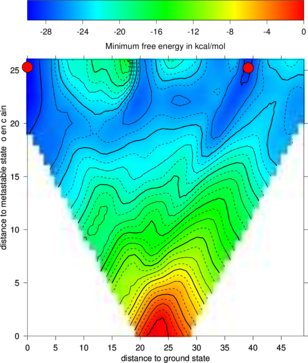
\includegraphics{Figs/2dfold_out_m.png}
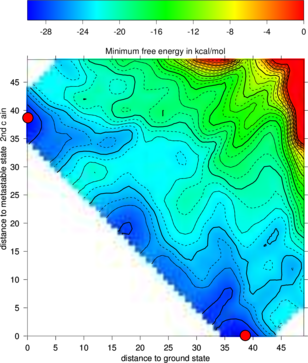
\includegraphics{Figs/2dfold_2_out_m.png}

\subsubsection{barriers \& treekin}{barriers \& treekin}\label{barriers-treekin}

The following assumes you have the barriers and treekin programs
installed. If not, the current release can be found at
\url{http://www.tbi.univie.ac.at/RNA/Barriers/}. Installation proceeds
as shown for the ViennaRNA Package in section
\hyperref[x1-80002.4]{2.4}. One problem that often occurs during treekin
installation is the dependency on \texttt{blas} and \texttt{lapack}
packages which is not carefully checked. For further information
according to the barriers and treekin program also see the website.

\textbf{A short recall on howto install/compile a program}\\
1. Get the barriers source from
\url{http://www.tbi.univie.ac.at/RNA/Barriers/} 2. extract the archive
and go to the directory

\begin{verbatim}
``` {.commands}
$ tar -xzf Barriers-1.5.2.tar.gz
$ cd Barriers-1.5.2
```

</div>
\end{verbatim}

\begin{enumerate}
\def\labelenumi{\arabic{enumi}.}
\setcounter{enumi}{2}
\tightlist
\item
  use the \texttt{-\/-prefix} option to install in your \texttt{Progs}
  directory

\begin{verbatim}
$ ./configure --prefix=$HOME/Tutorial/Progs/barriers-1.5.2
\end{verbatim}
\item
  make install

\begin{verbatim}
$ make
$ make install
\end{verbatim}
\end{enumerate}

Now barriers is ready to use. Apply the same steps to install treekin.
\texttt{Note:} Copy the barriers and treekin binaries to your
\texttt{bin} folder or add the path to your \texttt{PATH} variable.

\textbf{Calculate the Barrier Tree}\\

\begin{verbatim}
$ echo UCCACGGCUGUUAGUGGAUAACGGC | RNAsubopt --noLP -s -e 10 > barseq.sub
$ barriers -G RNA-noLP --bsize --rates < barseq.sub > barseq.bar
\end{verbatim}

You can restrict the number of local minima using the \texttt{barriers}
command-line option \texttt{-\/-max} followed by a number. The option
\texttt{-G\ RNA-noLP} instructs barriers that the input consists of RNA
secondary structures without isolated basepairs. \texttt{-\/-bsize} adds
size of the gradient basins and \texttt{-\/-rates} tells barriers to
compute rates between macro states/basins for use with treekin. Another
useful options is \texttt{-\/-minh} to print only minima with a barrier
\(> dE\). Look at the output file \texttt{less\ -S\ barseq.bar}. Use the
arrow keys to navigate.

\begin{verbatim}
  UCCACGGCUGUUAGUGGAUAACGGC
1 (((((........))))).......  -6.90    0  10.00    115     0  -7.354207     23  -7.012023
2 ......(((((((.....)))))))  -6.80    1   9.30     32    58  -6.828221     38  -6.828218
3 (((...(((...)))))).......  -0.80    1   0.90      1    10  -0.800000      9  -1.075516
4 ....((..((((....)))).))..  -0.80    1   2.70      5    37  -0.973593     11  -0.996226
5 .........................   0.00    1   0.40      1    14  -0.000000     26  -0.612908
6 ......(((....((.....)))))   0.60    2   0.40      1    22   0.600000      3   0.573278
7 ......((((((....)))...)))   1.00    1   1.50      1    95   1.000000      2   0.948187
8 .((....((......)).....)).   1.40    1   0.30      1    30   1.400000      2   1.228342
\end{verbatim}

The first row holds the input sequence, the successive list the local
minima ascending in energy. The meaning of the first 5 columns is as
follows

\begin{enumerate}
\def\labelenumi{\arabic{enumi}.}
\tightlist
\item
  label (number) of the local minima (1=MFE)
\item
  structure of the minimum
\item
  free energy of the minimum
\item
  label of deeper local minimum the current minimum merges with (note
  that the \texttt{MFE} has no deeper local minimum to merge with)
\item
  height of the energy barrier to the local minimum to merge with
\item
  numbers of structures in the basin we merge with
\item
  number of basin which we merge to
\item
  free energy of the basin
\item
  number of structures in this basin using gradient walk
\item
  gradient basin (consisting of all structures where gradientwalk ends
  in the minimum)
\end{enumerate}

\textbf{aCalculate The Barrier Tree}\\

\begin{figure}[htbp]
\centering

\includegraphics{Figs/tree.png}
\caption{pict}
\end{figure}

\texttt{barriers} produced two additional files, the \texttt{PostScript}
file \texttt{tree.eps} which represents the basic information of the
\texttt{barseq.bar} file visually (look at the file e.g.
\texttt{gv\ tree.eps}) and a text file \texttt{rates.out} which holds the
matrix of transition probabilities between the local minima.

\textbf{Simulating the Folding Kinetics}\\
 The program \texttt{treekin} is used to simulate the evolution over
time of the population densities of local minima starting from an
initial population density distribution \(p0\) (given on the
command-line) and the transition rate matrix in the file
\texttt{rates.out}.

\begin{verbatim}
$ treekin -m I --p0 5=1 < barseq.bar | xmgrace -log x -nxy -
\end{verbatim}

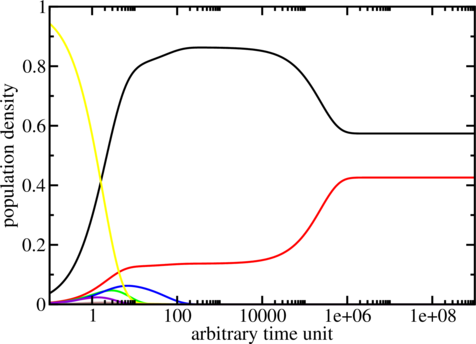
\includegraphics{Figs/FOO.png}

\includegraphics{Figs/FOO_dp.png}

The simulation starts with all the population density in the open chain
(local minimum 5, see \texttt{barseq.bar}). Over time the population
density of this state decays (yellow curve) and other local minima get
populated. The simulation ends with the population densities of the
thermodynamic equilibrium in which the MFE (black curve) and local
minimum 2 (red curve) are the only ones populated. (Look at the dot plot
of the sequence created with \texttt{RNAsubopt} and \texttt{RNAfold}!)

\subsection{Sequence Design}{Sequence Design}\label{sequence-design}

\subsubsection{The Program \texttt{RNAinverse}}{The Program RNAinverse}\label{the-program-rnainverse}

\texttt{RNAinverse} searches for sequences folding into a predefined
structure, thereby inverting the folding algorithm. Input consists of
the target structures (in dot-bracket notation) and a starting sequence,
which is optional.\\
Lower case characters in the start sequence indicate fixed positions,
i.e.~they can be used to add sequence constraints. '\texttt{N}'s in the
starting sequence will be replaced by a random nucleotide. For each
search the best sequence found and its Hamming distance to the start
sequence are printed to \emph{stdout}. If the the search was
unsuccessful a structure distance to the target is appended.\\
 By default the program stops as soon as it finds a sequence that has the
target as MFE structure. The option \texttt{-Fp} switches
\texttt{RNAinverse} to the partition function mode where the probability
of the target structure
\(\left. \exp\left( - E\left( S \right)\slash RT \right)\slash Q \right.\)
is maximized. This tends to produce sequences with a more well-defined
structure. This probability is written in dot-brackets after the found
sequence and Hamming distance. With the option \texttt{-R} you can
specify how often the search should be repeated.

\textbf{Sequence Design}\\
1. Prepare an input file \texttt{inv.in} containing the target structure
and sequence constraints

\begin{verbatim}
``` {.commands}
  (((.(((....))).)))
  NNNgNNNNNNNNNNaNNN
```
\end{verbatim}

\begin{enumerate}
\def\labelenumi{\arabic{enumi}.}
\setcounter{enumi}{1}
\tightlist
\item
  Design sequences using RNAinverse

\begin{verbatim}
$ RNAinverse < inv.in
      GGUgUUGGAUCCGAaACC    5

$ RNAinverse -R5 -Fp < inv.in
      GGUgUGAACCCUCGaACC    5
      GGCgCCCUUUUGGGaGCC   12  (0.967418)
      CUCgAUCUCACGAUaGGG    6
      GGCgCCCGAAAGGGaGCC   13  (0.967548)
      GUUgAGCCCAUGCUaAGC    6
      GGCgCCCUUAUGGGaGCC   10  (0.967418)
      CGGgUGUUGUGACAaCCG    5
      GCGgGUCGAAAGGCaCGC   12  (0.925482)
      GCCgUAUCCGGGUGaGGC    6
      GGCgCCCUUUUGGGaGCC   13  (0.967418)
\end{verbatim}
\end{enumerate}

The output consists of the calculated sequence and the number of
mutations needed to get the MFE-structure from the start sequence (start
sequence not shown). Additionaly, with the partition function folding
(\texttt{-Fp}) set, the second output is another refinement so that the
ensemble preferes the MFE and folds into your given structure with a
distinct probability, shown in brackets.\\
 Another useful program for inverse folding is \texttt{RNA\ designer},
see \url{http://www.rnasoft.ca/}. RNA Designer takes a secondary
structure description as input and returns an RNA strand that is likely
to fold in the given secondary structure.

The \texttt{sequence\ design\ application} of the
\texttt{ViennaRNA\ Design\ Webservices}, see
\url{http://nibiru.tbi.univie.ac.at/rnadesign/index.html} uses a
different approach, allowing for more than one secondary structure as
input. For more detail read the online Documentation and the next
section of this tutorial.

\subsubsection{switch.pl}{switch.pl}\label{switch.pl}

The \texttt{switch.pl} script can be used to design bi-stable
structures, i.e.~structures with two almost equally good foldings. For
two given structures there are always a lot of sequences compatible with
both structures. If both structures are reasonably stable you can find
sequences where both target structures have almost equal energy and all
other structures have much higher energies. Combined with RNAsubopt,
barriers and treekin, this is a very useful tool for designing
RNAswitches.\\
The input requires two structures in dot-bracket notation and
additionally you can add a sequence. It is also possible to calculate
the switching function at two different temperatures with option
\texttt{-T} and \texttt{-T2}.

\textbf{Designing a Switch}\\
 Now we try to create an RNA switch using \texttt{switch.pl}. First we
create our inputfile, then invoke the program using ten optimization runs
(\texttt{-n\ 10}) and do not allow lonely pairs. Write it out to
\texttt{switch.out}

\begin{verbatim}
switch.in
    ((((((((......))))))))....((((((((.......))))))))
    ((((((((((((((((((........)))))))))))))))))).....

$ switch.pl -n 10 --noLP < switch.in > switch.out
\end{verbatim}

\texttt{switch.out} should look similar like this, the first block
represents our bi-stable structures in random order, the second block
shows the resulting sequences ordered by their score.

\begin{verbatim}
$ less switch.out

GGGUGGACGUUUCGGUCCAUCCUUACGGACUGGGGCGUUUACCUAGUCC   0.9656
CAUUUGGCUUGUGUGUCGAAUGGCCCCGGUACGUAGGCUAAAUGUACCG   1.2319
GGGGGGUGCGUUCACACCCCUCAUUUGGUGUGGAUGUGCUUUCUACACU   1.1554
[...]
the resulting sequences are:
CAUUUGGCUUGUGUGUCGAAUGGCCCCGGUACGUAGGCUAAAUGUACCG   1.2319
GGGGGGUGCGUUCACACCCCUCAUUUGGUGUGGAUGUGCUUUCUACACU   1.1554
CGGGUUGUAACUGGAUAGCCUGGAAACUGUUUGGUUGUAAUCCGAACAG   1.0956
[...]
\end{verbatim}

Given all 10 suggestions in our \texttt{switch.out}, we select the one
with the best score with some command line tools to use it as an
\texttt{RNAsubopt} input file and build up the barriers tree.

\begin{verbatim}
$ tail -10 switch.out | awk '{print($1)}'  | head -n 1 > subopt.in
$ RNAsubopt --noLP -s -e 25 < subopt.in > subopt.out
$ barriers -G RNA-noLP --bsize --rates --minh 2 --max 30 < subopt.out > barriers.out
\end{verbatim}

\texttt{tail\ -10} cuts the last 10 lines from the \texttt{switch.out}
file and pipes them into an \texttt{awk} script. The function
\texttt{print(\$1)} echoes only the first column and this is piped into
the \texttt{head} program where the first line, which equals the best
scored sequence, is taken and written into \texttt{subopt.in}. Then
\texttt{RNAsubopt} is called to process our sequence and write the
output to another file which is the input for the barriers calculation.\\
 Below you find an example of the barriertree calculation above done with
the right settings (connected root) on the left side and the wrong
\texttt{RNAsubobt\ -e} value on the right. Keep in mind that
\texttt{switch.pl} performs an stochastic search and the output
sequences are different every time because there are a lot of sequences
which fit the structure and switch calculates a new one everytime. Simply
try to make sure.\\
 
\includegraphics{Figs/switch_barriertree.png}

\includegraphics{Figs/switch_barriertree_e13.png}
left: Barriers tree as it should look like, all branches connected to
the main root right: disconnected tree due to a too low
\texttt{energy\ range\ (-e)} parameter set in \texttt{RNAsubopt}.\\
 Be careful to set the range -e high enough, otherwise we get a problem
when calculation the kinetics using treekin. Every branch should be
somehow connected to the main root of the tree. Try \texttt{-e\ 20} and
\texttt{-e\ 30} to see the difference in the trees and choose the optimal
value. By using \texttt{-\/-max\ 30} we shorten our tree to focus only
on the lowest minima. We then select a branch preferably outside of the
two main branches, here branch 30 (may differ from your own calculation).
Look at the barrier tree to find the best branch to start and replace
\texttt{30} by the branch you would choose. Now use treekin to plot
concentration kinetics and think about the graph you just created.

\begin{verbatim}
$ treekin -m I --p0 30=1  < barriers.out > treekin.out
$ xmgrace -log x -nxy treekin.out
\end{verbatim}

The graph could look like the one below, remember everytime you use
\texttt{switch.pl} it can give you different sequences so the output
varies too. Here the one from the example.

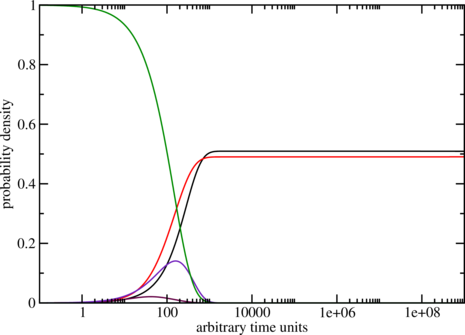
\includegraphics{Figs/switch_treekin.png}\\

\subsection{RNA-RNA Interactions}{RNA-RNA Interactions}\label{rna-rna-interactions}

A common problem is the prediction of binding sites between two RNAs, as
in the case of miRNA-mRNA interactions. Following tools of the
\texttt{ViennaRNA\ Package} can be used to calculate base pairing
probabilities.

\subsubsection{The Program \texttt{RNAcofold}}{The Program RNAcofold}\label{the-program-rnacofold}

\texttt{RNAcofold} works much like \texttt{RNAfold} but uses two RNA
sequences as input which are then allowed to form a dimer structure. In
the input the two RNA sequences should be concatenated using the
`\texttt{\&}' character as separator. As in \texttt{RNAfold} the
\texttt{-p} option can be used to compute partition function and base
pairing probabilities.\\
Since dimer formation is concentration dependent, \texttt{RNAcofold} can
be used to compute equilibrium concentrations for all five monomer and
(homo/hetero)-dimer species, given input concentrations for the monomers
(see the \texttt{man} page for details).

\textbf{Two Sequences one Structure}\\
1. Prepare a sequence file (\texttt{t.seq}) for input that looks like
this

\begin{verbatim}
``` {.commands}
>t
GCGCUUCGCCGCGCGCC&GCGCUUCGCCGCGCGCA
```

</div>
\end{verbatim}

\begin{enumerate}
\def\labelenumi{\arabic{enumi}.}
\setcounter{enumi}{1}
\tightlist
\item
  Compute the \texttt{MFE} and the ensemble properties
\item
  Look at the generated PostScript files \texttt{t\_ss.ps} and
  \texttt{t\_dp.ps}
\end{enumerate}

\begin{verbatim}
$ RNAcofold -p < t.seq
>t
GCGCUUCGCCGCGCGCC&GCGCUUCGCCGCGCGCA
((((..((..((((...&))))..))..))))... (-17.70)
((((..{(,.((((,,.&))))..}),.)))),,. [-18.26]
frequency of mfe structure in ensemble 0.401754 , delta G binding= -3.95
\end{verbatim}

\textbf{Secondary Structure Plot and Dot Plot}\\
 
\includegraphics{Figs/t_ss.png}

\includegraphics{Figs/t_dp.png}\\
In the dot plot a cross marks the chain break between the two
concatenated sequences.

\subsubsection{Concentration Dependency}{Concentration Dependency}\label{concentration-dependency}

Cofolding is an intermolecular process, therefore whether duplex
formation will actually occur is concentration dependent. Trivially, if
one of the molecules is not present, no dimers are going to be formed.
The partition functions of the molecules give us the equilibrium
constants:
-------------------------------------------------------------------------------------------------------------------------------------------
\[K_{AB} = \frac{\left\lbrack {AB} \right\rbrack}{\left\lbrack A \right\rbrack\left\lbrack B \right\rbrack} = \frac{Z_{AB}}{Z_{A}Z_{B}}\]
-------------------------------------------------------------------------------------------------------------------------------------------

with these and mass conservation, the equilibrium concentration of
homodimers, heterodimers and monomers can be computed in dependence of
the start concentrations of the two molecules. This is most easily done
by creating a file with the initial concentrations of molecules \(A\) and
\(B\) in two columns:\\
 \[\begin{array}{llll}
{\left\lbrack a_{1} \right\rbrack\left( \left\lbrack mol\slash l \right\rbrack \right)} & {\left\lbrack b_{1} \right\rbrack\left( \left\lbrack mol\slash l \right\rbrack \right)} & & \\
{\left\lbrack a_{2} \right\rbrack\left( \left\lbrack mol\slash l \right\rbrack \right)} & {\left\lbrack b_{2} \right\rbrack\left( \left\lbrack mol\slash l \right\rbrack \right)} & & \\
 \vdots & & & \\
{\left\lbrack a_{n} \right\rbrack\left( \left\lbrack mol\slash l \right\rbrack \right)} & {\left\lbrack b_{n} \right\rbrack\left( \left\lbrack mol\slash l \right\rbrack \right)} & & \\
\end{array}\]

\textbf{Concentration Dependency}\\
1. Prepare a concentration file for input with this little perl script

\begin{verbatim}
``` {.commands}
$ perl -e '$c=1e-07; do {print "$c\t$c\n"; $c*=1.71;} while $c<0.2' > concfile
```

This script creates a file displaying values from 1e-07 to just below
0.2, with 1.71-fold steps in between. For convenience, concentration
of molecule A is the same as concentration of molecule B in
each row. This will facilitate visualization of the results.
\end{verbatim}

\begin{enumerate}
\def\labelenumi{\arabic{enumi}.}
\setcounter{enumi}{1}
\tightlist
\item
  Compute the \texttt{MFE}, the ensemble properties and the
  concentration dependency of hybridization.

\begin{verbatim}
$ RNAcofold -f concfile < t.seq > cofold.out
\end{verbatim}
\item
  Look at the generated output with
\begin{verbatim}
$ less cofold.out
\end{verbatim}
\end{enumerate}

\begin{verbatim}
[...]
Free Energies:
AB              AA              BB              A               B
-18.261023      -17.562553      -18.274376      -7.017902       -7.290237
Initial concentrations          relative Equilibrium concentrations
A                B               AB              AA              BB              A               B
1e-07           1e-07           0.00003         0.00002         0.00002         0.49994         0.49993
[...]
\end{verbatim}

The five different free energies were printed out first, followed by a list
of all the equilibrium concentrations, where the first two columns denote
the initial (absolute) concentrations of molecules \(A\) and \(B\),
respectively. The next five columns denote the equilibrium concentrations
of dimers and monomers, relative to the total particle number. (Hence,
the concentrations don't add up to one, except in the case where no
dimers are built -- if you want to know the fraction of particles in a
dimer, you have to take the relative dimer concentrations times 2).\\
Since relative concentrations of species depend on two independent
values - initial concentration of A as well as initial concentration of
B - it is not trivial to visualize the results. For this reason we used
the same concentration for A and for B. Another possibility would be to
keep the initial concentration of one molecule constant. As an example
we show the following plot of \(t.seq\). Now we use some commandline
tools to render our plot. We use \texttt{tail\ -n\ +11} to show all
lines starting with line 11 (1-10 are cut) and pipe it into an
\texttt{awk} command, which prints every column but the first from our
input. This is then piped to \texttt{xmgrace}. With
\texttt{-log\ x\ -nxy\ -} we tell it to plot the x axis in logarithmic
scale and to read data file in X Y1 Y2 \ldots{} format.

\begin{verbatim}
$ tail -n +11 cofold.out | awk '{print $2, $3, $4, $5, $6, $7}' | xmgrace -log x -nxy -
\end{verbatim}

\textbf{Concentration Dependency plot}\\

\begin{center}\rule{0.5\linewidth}{\linethickness}\end{center}

\begin{figure}[htbp]
\centering
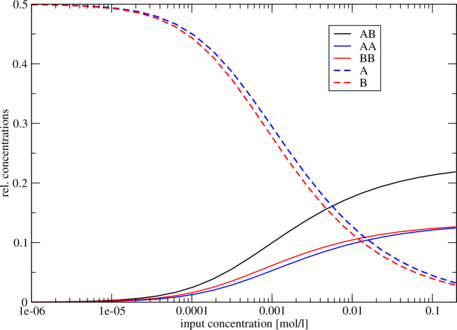
\includegraphics{Figs/tconcdep.png}
\caption{pict}
\end{figure}

\begin{center}\rule{0.5\linewidth}{\linethickness}\end{center}

\(\Delta G_{\text{binding}} = - 5.01\) kcal/mol

\begin{verbatim}
  sequences:GCGCUUCGCCGCGCGCG&GCGCUUCGCCGCGCGCG
\end{verbatim}

Since the two sequences are almost identical, the monomer and homo-dimer
concentrations behave very similarly. In this example, at a
concentration of about 1 mmol 50\% of the molecule is still in monomer
form.

\subsubsection{Finding potential binding sites with RNAduplex}{Finding potential binding sites with RNAduplex}\label{finding-potential-binding-sites-with-rnaduplex}

If the sequences are very long (many kb)\texttt{RNAcofold} is too slow
to be useful. The \texttt{RNAduplex} program is a fast alternative, that
works by predicting \emph{only} intermolecular base pairs. It's almost
as fast as simple sequence alignment, but much more accurate than a
\texttt{BLAST} search.

The example below searches the 3' UTR of an mRNA for a miRNA binding
site.

\textbf{Binding site prediction with RNAduplex}\\
 The file \texttt{duplex.seq} contains the 3'UTR of NM\_024615 and the
microRNA mir-145.

\begin{verbatim}
$ RNAduplex < duplex.seq
>NM_024615
>hsa-miR-145
.(((((.(((...((((((((((.&)))))))))))))))))).  34,57  :   1,19  (-21.90)
\end{verbatim}

Most favorable binding has an interaction energy of -21.90 kcal/mol and
pairs up on positions 34-57 of the UTR with positions 1-22 of the
miRNA.\\
 \texttt{RNAduplex} can also produce alternative binding sites,
e.g.~running \texttt{RNAduplex\ -e\ 10} would list all binding sites
within 10 kcal/mol of the best one.

Since \texttt{RNAduplex} forms only intermolecular pairs, it neglects
the competition between intramolecular folding and hybridization. Thus,
it is recommended to use \texttt{RNAduplex} as a pre-filter and analyse
good \texttt{RNAduplex} hits additionally with \texttt{RNAcofold} or
\texttt{RNAup}. Using the example above, running \texttt{RNAup} will
yield:

\begin{verbatim}
$ RNAup -b < duplex.seq

>NM_024615
>hsa-miR-145
(((((((&)))))))  50,56  :   1,7   (-8.41 = -9.50 + 0.69 + 0.40)
GCUGGAU&GUCCAGU
RNAup output in file: hsa-miR-145_NM_024615_w25_u1.out
\end{verbatim}

The free energy of the duplex is -9.50 kcal/mol and shows a discrepancy
to the structure and energy value computed by \texttt{RNAduplex}
(differences may arise from the fact that RNAup computes partition
functions rather than optimal structures). However, the total free
energy of binding is less favorable (-8.41 kcal/mol), since it includes
the energetic penalty for opening the binding site on the mRNA (0.69
kcal/mol) and miRNA (0.40 kcal/mol). The \texttt{-b} option includes the
probability of unpaired regions in both RNAs.

You can also run \texttt{RNAcofold} on the example to see the complete
structure after hybridization (neither \texttt{RNAduplex} nor
\texttt{RNAup} produce structure drawings). Note however, that the input
format for \texttt{RNAcofold} is different. An input file suitable for
\texttt{RNAcofold} has to be created from the \texttt{duplex.seq} file
first (use any text editor).\\
 As a more difficult example, let's look at the interaction of the
bacterial smallRNA RybB and its target mRNA ompN. First we'll try
predicting the binding site using RNAduplex:

\begin{verbatim}
$ RNAduplex < RybB.seq
>RybB
>ompN
.((((..((((((.(((....((((((((..(((((.((..((.((....((((..(((((((((((..((((((&
.))))))..))))))).)))).....))))....)).)).)).))).))..))))........))))..))).)))))).)))).
 5,79  :  80,164 (-34.60)
\end{verbatim}

Note, that the predicted structure spans almost the full length of the
RybB small RNA. Compare the predicted interaction to the structures
predicted for RybB and ompN alone, and ask yourself whether the
predicted interaction is indeed plausible.

Below the structure of ompN on the left and RybB on the right side. The
respective binding regions predicted by RNAduplex are marked in red.

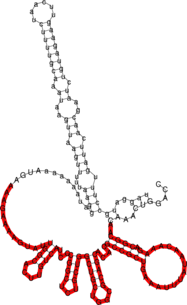
\includegraphics{Figs/ompN_ss.png}

\includegraphics{Figs/RybB_ss.png}

\begin{verbatim}
GCCAC-----TGCTTTTCTTTGATGTCCCCATTTT-GTGGA-------GC-CCATCAACCCCGCCATTTCGGTT---CAAG-GTTGGTGGGTTTTTT
 |||      ||||  |||||| |||    ||||| ||||        || ||| || ||  ||    ||||     |||| ||  |||  |||||| -40.30
AGGTCAAACAACGGC-AGAAACAATATT--TAAAGTCGCCGCACACGACGCGGTCGTCGGT-CGTCTCGGCCCTACTGTTCACGGTTATGAAAAGAAACC-3'
\end{verbatim}

Compare the \texttt{RNAduplex} prediction with the interaction predicted
by \texttt{RNAcofold}, \texttt{RNAup} and the handcrafted prediction you
see above.

\begin{figure}[htbp]
\centering
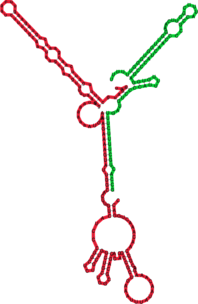
\includegraphics{Figs/OmpN_cofold.png}
\caption{pict}
\end{figure}

\subsection{Consensus Structure Prediction}{Consensus Structure Prediction}\label{consensus-structure-prediction}

Sequence co-variations are a direct consequence of RNA base pairing
rules and can be deduced to alignments. RNA helices normally contain
only 6 out of the 16 possible combinations: the Watson-Crick pairs GC,
CG, AU, UA, and the somewhat weaker wobble pairs GU and UG. Mutations in
helical regions therefore have to be correlated. In particular we often
find ``compensatory mutations'' where a mutation on one side of the helix
is compensated by a second mutation on the other side, e.g.~a
C\(\cdot\)G pair changes into a U\(\cdot\)A pair. Mutations where only
one pairing partner changes (such as C\(\cdot\)G to U\(\cdot\)G) are
termed ``consistent mutations''.

\subsubsection{The Program \texttt{RNAalifold}}{The Program RNAalifold}\label{the-program-rnaalifold}

\texttt{RNAalifold} generalizes the folding algorithm for sequence
alignments, treating the entire alignment as a single ``generalized
sequence''. To assign an energy to a structure on such a generalized
sequence, the energy is simply averaged over all sequences in the
alignment. This average energy is augmented by a covariance term, that
assigns a bonus or penalty to every possible base pair
\(\left( {i,j} \right)\) based on the sequence variation in columns
\(i\) and \(j\) of the alignment.\\
Compensatory mutations are a strong indication of structural
conservation, while consistent mutations provide a weaker signal. The
covariance term used by \texttt{RNAalifold} therefore assigns a bonus of
1 kcal/mol to each consistent and 2 kcal/mol for each compensatory
mutation. Sequences that cannot form a standard base pair incur a
penalty of \(- 1\) kcal/mol. Thus, for every possible consensus pair
between two columns \(i\) and \(j\) of the alignment a covariance score
\(C_{ij}\) is computed by counting the fraction of sequence pairs
exhibiting consistent and compensatory mutations, as well as the
fraction of sequences that are inconsistent with the pair. The weight of
the covariance term relative to the normal energy function, as well as
the penalty for inconsistent mutations can be changed via command line
parameters.\\
 Apart from the covariance term, the folding algorithm in
\texttt{RNAalifold} is essentially the same as for single sequence
folding. In particular, folding an alignment containing just one
sequence will give the same result as single sequence folding using
\texttt{RNAfold}. For \(N\) sequences of length \(n\) the required CPU
time scales as
\(\mathcal{\mathcal{O}}\left( {N \cdot n^{2} + n^{3}} \right)\) while
memory requirements grow as the square of the sequence length. Thus
\texttt{RNAalifold} is in general faster than folding each sequence
individually. The main advantage, however, is that the accuracy of
consensus structure predictions is generally much higher than for single
sequence folding, where typically only between 40\% and 70\% of the base
pairs are predicted correctly.\\
 Apart from prediction of \texttt{MFE} structures \texttt{RNAalifold}
also implements an algorithm to compute the partition function over all
possible (consensus) structures and the thermodynamic equilibrium
probability for each possible pair. These base pairing probabilities are
useful to see structural alternatives, and to distinguish well defined
regions, where the predicted structure is most likely correct, from
ambiguous regions.\\
 As a first example we'll produce a consensus structure prediction for
the following four tRNA sequences.

\begin{verbatim}
$ cat four.seq
\end{verbatim}

\begin{verbatim}
>M10740 Yeast-PHE
GCGGAUUUAGCUCAGUUGGGAGAGCGCCAGACUGAAGAUUUGGAGGUCCUGUGUUCGAUCCACAGAAUUCGCA
>K00349 Drosophila-PHE
GCCGAAAUAGCUCAGUUGGGAGAGCGUUAGACUGAAGAUCUAAAGGUCCCCGGUUCAAUCCCGGGUUUCGGCA
>K00283 Halobacterium volcanii Lys-tRNA-1
GGGCCGGUAGCUCAUUUAGGCAGAGCGUCUGACUCUUAAUCAGACGGUCGCGUGUUCGAAUCGCGUCCGGCCCA
>AF346993
CAGAGUGUAGCUUAACACAAAGCACCCAACUUACACUUAGGAGAUUUCAACUUAACUUGACCGCUCUGA
\end{verbatim}

\texttt{RNAalifold} uses aligned sequences as input. Thus, our first step
will be to align the sequences. We use \texttt{clustalw2} in this
example, since it's one of the most widely used alignment programs and
has been shown to work well on structural RNAs. Other alignment programs
can be used (including programs that attempt to do structural alignment
of RNAs), but the resulting multiple sequence alignment must be in
\texttt{Clustal} format. Get \texttt{clustalw2} and install it as you
have done it with the other packages:
\url{http://www.clustal.org/clustal2}

\textbf{Consensus Structure from related Sequences}\\
1. Prepare a sequence file (use file \texttt{four.seq} and copy it to your
working directory) 2. Align the sequences 3. Compute the consensus
structure from the alignment 4. Inspect the output files
\texttt{alifold.out}, \texttt{alirna.ps}, \texttt{alidot.ps} 5. For
comparison fold the sequences individually using \texttt{RNAfold}

\begin{verbatim}
$ clustalw2 four.seq > four.out
\end{verbatim}

\texttt{Clustalw2} creates two more output files, \texttt{four.aln} and
\texttt{four.dnd}. For \texttt{RNAalifold} you need the\texttt{.aln}
file.

\begin{verbatim}
$ RNAalifold -p four.aln
$ RNAfold -p < four.seq
\end{verbatim}

\texttt{RNAalifold} output:

\begin{verbatim}
__GCCGAUGUAGCUCAGUUGGG_AGAGCGCCAGACUGAAAAUCAGAAGGUCCCGUGUUCAAUCCACGGAUCCGGCA__
..(((((((..((((.........)))).(((((.......))))).....(((((.......))))))))))))...
 minimum free energy = -15.12 kcal/mol (-13.70 +  -1.43)
..(((((({..((((.........)))).(((((.......))))).....(((((.......)))))}))))))...
 free energy of ensemble = -15.75 kcal/mol
 frequency of mfe structure in ensemble 0.361603
..(((((((..((((.........)))).(((((.......))))).....(((((.......))))))))))))... -15.20 {-13.70 +  -1.50}
\end{verbatim}

\texttt{RNAfold} output:

\begin{verbatim}
>M10740 Yeast-PHE
GCGGAUUUAGCUCAGUUGGGAGAGCGCCAGACUGAAGAUUUGGAGGUCCUGUGUUCGAUCCACAGAAUUCGCA
((((((((........((((.((((((..((((...........))))..))))))..))))..)))))))). (-21.60)
((((((({...,,.{,((((.((((((..((((...........))))..))))))..))))),)))))))). [-23.20]
((((((((.........(((.((((((..((((...........))))..))))))..)))...)))))))). {-20.00 d=9.63}
 frequency of mfe structure in ensemble 0.0744065; ensemble diversity 15.35
>K00349 Drosophila-PHE
[...]
\end{verbatim}

The output contains a consensus sequence and the consensus structure in
dot-bracket notation. The consensus structure has an energy of
\(- 15.12\)~kcal/mol, which in turn consists of the average free energy
of the structure \(- 13.70\)~kcal/mol and the covariance term
\(- 1.43\)~kcal/mol. The strongly negative covariance term shows that
there must be a fair number of consistent and compensatory mutations,
but in contrast to the average free energy it's not meaningful in the
biophysical sense.

Compare the predicted consensus structure with the structures predicted
for the individual sequences using \texttt{RNAfold}. How often is the
correct ``clover-leaf'' shape predicted?

For better visualization, a structure annotated alignment or color
annotated structure drawing can be generated by using the
\texttt{-\/-aln} and \texttt{-\/-color} options of \texttt{RNAalifold}.

\begin{verbatim}
$ RNAalifold --color --aln four.aln
$ gv aln.ps &
$ gv alirna.ps &
\end{verbatim}

\textbf{\texttt{RNAalifold} Output Files}\\

\begin{verbatim}
4 sequence; length of alignment 78
alifold output
   6    72  0  99.8%   0.007 GC:2    GU:1    AU:1
  33    43  0  98.9%   0.033 GC:2    GU:1    AU:1
  31    45  0  99.0%   0.030 CG:3    UA:1
  15    25  0  98.9%   0.045 CG:3    UA:1
   5    73  1  99.7%   0.008 CG:2    GC:1
  13    27  0  99.1%   0.042 CG:4
  14    26  0  99.1%   0.042 UA:4
   4    74  1  99.5%   0.015 CG:3
[...]
\end{verbatim}

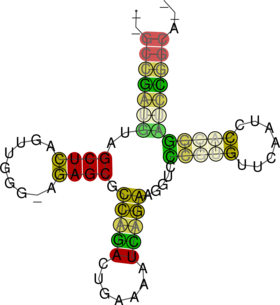
\includegraphics{Figs/alirna.png}
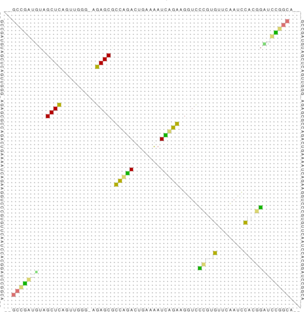
\includegraphics{Figs/alidot.png}

The last output file produced by \texttt{RNAalifold\ -p}, named
\texttt{alifold.out}, is a plain text file with detailed information on
all plausible base pairs sorted by the likelihood of the pair. In the
example above we see that the pair \(\left( {6,72} \right)\) has no
inconsistent sequences, is predicted almost with probability 1, and
occurs as a GC pair in two sequences, a GU pair in one, and a AU pair in
another.

\texttt{RNAalifold} automatically produces a drawing of the consensus
structure in Postscript format and writes it to the file
``\texttt{alirna.ps}''. In the structure graph consistent and
compensatory mutations are marked by a circle around the variable
base(s), i.e.~pairs where one pairing partner is encircled exhibit
consistent mutations, whereas pairs supported by compensatory mutations
have both bases marked. Pairs that cannot be formed by some of the
sequences are shown gray instead of black. In the example given, many
pairs show such inconsistencies. This is because one of the sequences
(AF346993) is not aligned well by \texttt{clustalw}.

Note, that subsequent calls to \texttt{RNAalifold} will overwrite any
existing output \texttt{alirna.ps} (\texttt{alidot.ps},
\texttt{alifold.out}) files in the current directory. Be sure to rename
any files you want to keep.

\textbf{Structure predictions for the individual sequences}\\
The consensus structure computed by \texttt{RNAalifold} will contain
only pairs that can be formed by most of the sequences. The structures
of the individual sequences will typically have additional base pairs
that are not part of the consensus structure. Moreover, ncRNA may
exhibit a highly conserved core structure while other regions are more
variable. It may therefore be desirable to produce structure predictions
for one particular sequence, while still using covariance information
from other sequences.

This can be accomplished by first computing the consensus structure for
all sequences using \texttt{RNAalifold}, then folding individual
sequences using \texttt{RNAfold\ -C} with the consensus structure as a
constraint. In constraint folding mode \texttt{RNAfold\ -C} allows only
base pairs to form which are compatible with the constraint structure.
This resulting structure typically contains most of the constraint (the
consensus structure) plus some additional pairs that are specific for
this sequence.

\textbf{Refolding Individual Sequences}\\
 The \texttt{refold.pl} (find it in the Progs folder) script removes gaps
and maps the consensus structure to each individual sequence.

\begin{verbatim}
$ RNAalifold  RNaseP.aln > RNaseP.alifold
$ gv alirna.ps
$ refold.pl RNaseP.aln RNaseP.alifold | head -3 > RNaseP.cfold
$ RNAfold -C --noLP < RNaseP.cfold > RNaseP.refold
$ gv E-coli_ss.ps
\end{verbatim}

If you compare the refolded structure ({{E-coli\_ss.ps}}) with the
structure you get by simply folding the E.coli sequence in the
RNaseP.seq file ({{RNAfold~--noLP}}) you find a clear rearrangement.

In cases where constrained folding results in a structure that is very
different from the consensus, or if the energy from constrained folding
is much worse than from unconstrained folding, this may indicate that
the sequence in question does not really share a common structure with
the rest of the alignment or is misaligned. One should then either
remove or re-align that sequence and recompute the consensus structure.

Note that since RNase P forms sizable pseudo-knots, a perfect prediction
is impossible in this case.

\subsection{Structural Alignments}{Structural Alignments}\label{structural-alignments}

\subsubsection{Manually correcting Alignments}{Manually correcting Alignments}\label{manually-correcting-alignments}

As the tRNA example above demonstrates, sequence alignments are often
unsuitable as a basis for determining consensus structures. As a last
resort, one may always try manually correcting an alignment. Sequence
editors that are structure-aware may help in this task. In particular
the SARSE \url{http://sarse.kvl.dk/} editor, and the \texttt{ralee-mode}
for emacs
\url{http://personalpages.manchester.ac.uk/staff/sam.griffiths-jones/software/ralee/}
are useful. After downloading the \texttt{ralee}-files extract them and
put them in a folder called
\texttt{\textasciitilde{}/Tutorial/Progs/ralee}. Now read the
\texttt{00README} file and follow the instructions. If you don't find an
``.emacs'' file in your home directory execute the following command to
copy it from the Data directory.\\

\begin{verbatim}
$ cp Data/dot.emacs ~/
\end{verbatim}

Next try correcting the \texttt{ClustalW} generated alignment
\texttt{(four.aln)} from the example above. For this we first have to
convert it to the Stockholm format. Fortunately the formats are similar.
Make a copy of the file add the correct header line and the consensus
structure from RNAalifold:

\begin{verbatim}
$ cp four.aln four.stk
$ emacs four.stk
  .....
$ cat four.stk
\end{verbatim}

The final alignment should look like:

\begin{verbatim}
# STOCKHOLM 1.0

K00349          --GCCGAAAUAGCUCAGUUGGG-AGAGCGUUAGACUGAAGAUCUAAAGGUCCCCGGUUCAAUCCCGGGUUUCGGCA--
K00283          GGGCCG--GUAGCUCAUUUAGGCAGAGCGUCUGACUCUUAAUCAGACGGUCGCGUGUUCGAAUC--GCGUCCGGCCCA
M10740          --GCGGAUUUAGCUCAGUUGGG-AGAGCGCCAGACUGAAGAUUUGGAGGUCCUGUGUUCGAUCCACAGAAUUCGCA--
AF346993        --CAGAGUGUAGCUUAAC---ACAAAGCACCCAACUUACACUUAGGAGAUUUCAACUUAACUUGACCGCUCUGA----
#=GC SS_cons    ..(((((((..((((.........)))).(((((.......))))).....(((((.......))))))))))))...
//
\end{verbatim}

Now use the functions under the edit menu to improve the alignment, the
coloring by structure should help to highlight misaligned positions.

\subsubsection{Automatic structural alignments}{Automatic structural alignments}\label{automatic-structural-alignments}

Next, we'll compute alignments using two structural alignment programs:
\texttt{LocARNA} and \texttt{T-Coffee}. \texttt{LocARNA} is an
implementation of the Sankoff algorithm for simultaneous folding and
alignment (i.e.~it will generate both alignment and consensus
structure). \texttt{T-Coffee} uses a progressive alignment algorithm.

Download \texttt{LocARNA} from
\url{http://www.bioinf.uni-freiburg.de/Software/LocARNA/}, extract and
install it in your \texttt{Progs} folder and eventually add it to your
path variable or copy it into the corresponding directory.

Both programs can read the fasta file \texttt{four.seq}.

\begin{verbatim}
$ mlocarna --alifold-consensus-dp four.seq
[...]
M10740             GCGGAUUUAGCUCAGUUGGG-AGAGCGCCAGACUGAAGAUUUGGAGGUCCUGUGUUCGAUCCACAGAAUUCGCA
K00349             GCCGAAAUAGCUCAGUUGGG-AGAGCGUUAGACUGAAGAUCUAAAGGUCCCCGGUUCAAUCCCGGGUUUCGGCA
K00283             GGGCCGGUAGCUCAUUUAGGCAGAGCGUCUGACUCUUAAUCAGACGGUCGCGUGUUCGAAUCGCGUCCGGCCCA
AF346993           CAGAGUGUAGCUUAAC---ACAAAGCACCCAACUUACACUUAGGAGAUU-UCAACUUAA-CUUGACCGCUCUGA
alifold            (((((((..((((.........)))).(((((.......))))).....(((((.......)))))))))))).
      (-52.53 = -21.58 + -30.95)
\end{verbatim}

\textbf{Install T-Coffee}\\
Get \texttt{T-Coffee} from the github page
\url{https://github.com/cbcrg/tcoffee}. There is a detailed information
how you should download and install the software in the given README.md.

Go to the \texttt{downloads} directory and use the provided installer by
typing

\begin{verbatim}
$ cd Tutorial/downloads
$ git clone git@github.com:cbcrg/tcoffee.git tcoffee
$ cd tcoffee/compile/
$ make t_coffee
$ cp t_coffee ~/Tutorial/Progs/
\end{verbatim}

Afterwards align the \texttt{four.seq} using \texttt{t\_coffee} and
compare the output with the one given by LocARNA.

\begin{verbatim}
$ t_coffee four.seq > t_coffee.out

 [t_coffee.out]
 CLUSTAL FORMAT for T-COFFEE 20150925_14:18 [http://www.tcoffee.org] [MODE:  ],
 CPU=0.00 sec, SCORE=739, Nseq=4, Len=74

 M10740          GCGGAUUUAGCUCAGUU-GGGAGAGCGCCAGACUGAAGAUUUGGAGGUCC
 K00349          GCCGAAAUAGCUCAGUU-GGGAGAGCGUUAGACUGAAGAUCUAAAGGUCC
 K00283          GGGCCGGUAGCUCAUUUAGGCAGAGCGUCUGACUCUUAAUCAGACGGUCG
 AF346993        CAGAGUGUAGCUUAAC---ACAAAGCACCCAACUUACACUUAGGAGAUUU
                   ***** *       * ***     ***     *     * *

 M10740          UGUGUUCGAUCCACAGAAUUCGCA
 K00349          CCGGUUCAAUCCCGGGUUUCGGCA
 K00283          CGUGUUCGAAUCGCGUCCGGCCCA
 AF346993        CAACUUAACUUGACCG--CUCUGA
                 **                 *
\end{verbatim}

Use RNAalifold to predict structures for all your alignments (ClustalW,
handcrafted, T-Coffee, and LocARNA) and compare them. The handcrafted and
LocARNA alignments should be essentially perfect.

Other interesting approaches to structural alignment include
\texttt{CMfinder}, \texttt{dynalign}, and \texttt{stemloc}.

\subsection{Noncoding RNA gene prediction}{Noncoding RNA gene prediction}\label{noncoding-rna-gene-prediction}

Prediction of ncRNAs is still a challenging problem in bioinformatics.
Unlike protein coding genes, ncRNAs do not have any statistically
significant features in primary sequences that could be used for reliable
prediction. A large class of ncRNAs, however, depend on a defined
secondary structure for their function. As a consequence, evolutionarily
conserved secondary structures can be used as characteristic signal to
detect ncRNAs. All currently available programs for \emph{de novo}
prediction make use of this principle and are therefore, by
construction, limited to structured RNAs.

\textbf{Programs to predict structural RNAs}\\
- \texttt{QRNA} (Eddy \& Rivas, 2001) - \texttt{ddbRNA} (di Bernardo,
Down \& Hubbard, 2003) - \texttt{MSARi} (Coventry, Kleitman \& Berger,
2004) - \texttt{AlifoldZ} (Washietl \& Hofacker, 2004) - \texttt{RNAz}
(Washietl, Hofacker \& Stadler, 2005) - \texttt{EvoFold} (Pedersen et
al, 2006)

\subsubsection{QRNA}{QRNA}\label{qrna}

\texttt{QRNA} analyzes pairwise alignments for characteristic patterns
of evolution. An alignment is scored by three probabilistic models: (i)
Position independent, (ii) coding, (iii) RNA. The independent and the
coding model is a pair hidden Markov model. The RNA model is a pair
stochastic context-free grammar. First, it calculates the \emph{prior
probability} that, given a model, the alignment is observed. Second, it
calculates the \emph{posterior probability} that, given an alignment, it
has been generated by one of the three models. The posterior
probabilities are compared to the position independent background model
and a ``winner'' is found. \texttt{QRNA} reads pairwise alignments in
MFASTA format (i.e.~FASTA format with gaps)

\textbf{Three competing models in QRNA}\\

\begin{figure}[htbp]
\centering
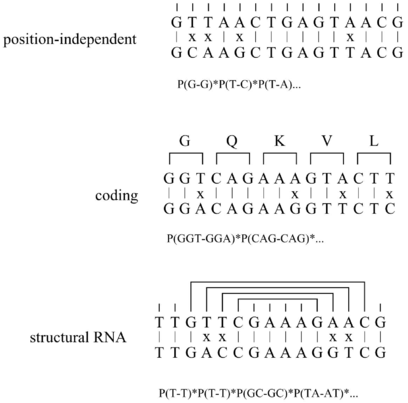
\includegraphics{Figs/qrna.png}
\caption{pict}
\end{figure}

\textbf{Installing and basic usage of QRNA}\\
- Use the files in \texttt{qrna-2.0.3d.tar.gz} located in the
\texttt{Data/programs}-folder shipped with the tutorial - don't forget
to set the \texttt{QRNADB} environment variable\\
 (e.g. {{export~QRNADB=\$HOME/Tutorial/Data/programs/qrna-2.0.3d/lib/}})
and add it to your \texttt{.bashrc} - follow the instructions in the
\texttt{INSTALL} document and make the binaries - create the directory
\texttt{\textasciitilde{}/Tutorial/Progs/qrna} and move the binaries
located in the \texttt{src/} sub-directory into this folder and add it
to your \texttt{.bashrc}\\
 (e.g.
{{export~PATH=\$\{HOME\}/Tutorial/Progs:\$\{PATH\}:\$\{HOME\}/Tutorial/Progs/qrna}})
- first read the help text (option \texttt{-h}). - for advanced use of
\texttt{QRNA} read the \texttt{userguide.pdf} shipped with the package
(in the \texttt{documentation} folder - \texttt{-a} tells \texttt{QRNA}
to print the alignment

\begin{verbatim}
$ eqrna -h
$ eqrna -a Data/qrna/tRNA.fa
$ eqrna -a Data/qrna/coding.fa
\end{verbatim}

\begin{verbatim}
[...]
Divergence time (variable): 0.214132 0.208107 0.203995
[alignment ID = 72.37 MUT = 23.68 GAP = 3.95]

length alignment: 76 (id=72.37) (mut=23.68) (gap=3.95)
posX: 0-75 [0-72](73) -- (0.18 0.30 0.36 0.16)
posY: 0-75 [0-75](76) -- (0.14 0.34 0.37 0.14)


          DA0780 GGGCTCGTAGCTCAGCT.GGAAGAGCGCGGCGTTTGCAACGCCGAGGCCT
          DA0940 GGGCCGGTAGCTCAGCCTGGGAGAGCGTCGGCTTTGCAAGCCGAAGGCCC

          DA0780 GGGGTTCAAATCCCCACGGGTCCA..
          DA0940 CGGGTTCGAATCCCGGCCGGTCCACC
[..]
\end{verbatim}

\subsubsection{AlifoldZ}{AlifoldZ}\label{alifoldz}

\texttt{AlifoldZ} is based on an old hypothesis: functional RNAs are
thermodynamically more stable than expected by chance. This hypothesis
can be statistically tested by calculating \(z\)-scores: Calculate the
MFE \(m\) of the native RNA and the mean \(\mu\) and standard deviation
\(\sigma\) of the background distribution of a large number of random
(shuffled) RNAs. The normalized \(z\)-score
\(\left. z = \left( {m - \mu} \right)\slash\sigma \right.\) expresses
how many standard deviations the native RNA is more stable than random
sequences. Unfortunately, most ncRNAs are not significantly more stable
than the background. See for example the distribution of \(z\)-scores of
some tRNAs, where the overlap of real (green bars) and shuffled (dashed
line) tRNAs is relatively high.

\textbf{z-score distribution of tRNAs}\\

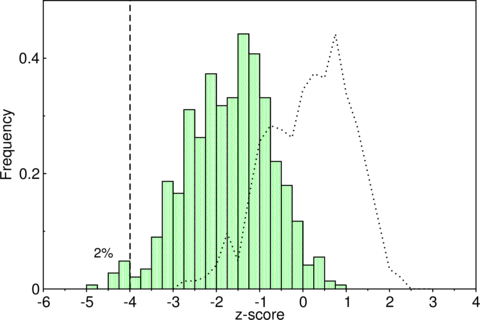
\includegraphics{Figs/trna-histo.png}\\
 The overlap of real (bars) and shuffled (dashed line) tRNAs is relatively
high.

\begin{center}\rule{0.5\linewidth}{\linethickness}\end{center}

\texttt{AlifoldZ} calculates \(z\)-scores for consensus structures
folded by \texttt{RNAalifold}. This significantly improves the detection
performance compared to single sequence folding.

\textbf{z-score distribution of tRNA consensus folds}\\

------------------------------------------------------------------------

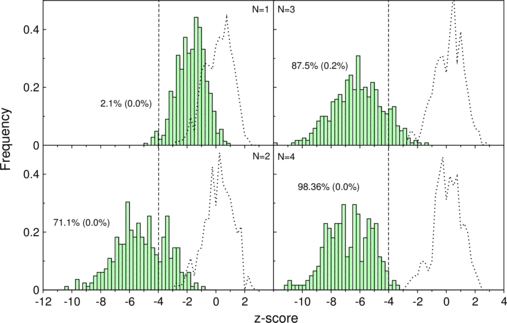
\includegraphics{Figs/histos.png}\\
 The separation of real and shuffled tRNAs gets evident with more
sequences in the alignment.

\begin{center}\rule{0.5\linewidth}{\linethickness}\end{center}

\textbf{Installation and basic usage of AlifoldZ}\\
- Use the tarball \texttt{alifoldz\_adopted.tar.gz} located in the
\texttt{Data/programs/}-folder shipped with the tutorial - Copy the files
into your \texttt{Progs} directory (It's just one single Perl script
which needs \texttt{RNAfold} and \texttt{RNAalifold} and an important
perl module located in the Math subdirectory)\\
 {{~\$~cp~-r~alifoldz.pl~Math/~\textasciitilde{}/Tutorial/Progs/}} - add
the perl module to your \texttt{PERL5LIB} variable in the
\texttt{.bashrc}\\
 {{~\$~export~PERL5LIB=\$HOME/Tutorial/Progs/:\$PERL5LIB}} - test the
tool

\begin{verbatim}
$ alifoldz.pl -h
$ alifoldz.pl < Data/alifoldz/miRNA.aln
$ alifoldz.pl -w 120 -x 100 < Data/alifoldz/unknown.aln
\end{verbatim}

\subsubsection{RNAz}{RNAz}\label{rnaz}

\hyperdef{}{textcolor1}{\label{textcolor1}}{* New version by Someone who
loves RNAz. This part of the tutorial is based on the RNAz 1.0 version
which is obsolete quite a while already!!! *}\\
\texttt{AlifoldZ} has some shortcomings that limits its usefulness in
practice: The \(z\)-scores are not deterministic, i.e.~you get a
different score each time you run \texttt{AlifoldZ}. To get stable
\(z\)-scores you need to sample a large number of random alignments
which is computationally expensive. Moreover, \texttt{AlifoldZ} is
extremely sensitive to alignment errors.

The program \texttt{RNAz} overcomes these problems by using a different
approach to asses a multiple sequence alignment for significant RNA
structures. It is based on two key innovations: (i) The structure
conservation index (SCI) to measure structural conservation in an
alignment and (ii) \(z\)-scores that are calculated by regression
without sampling. Both measures are combined to an overall score that is
used to classify an alignment as ``structured RNA'' or ``other''.

\textbf{The structure conservation index}\\

\begin{figure}[htbp]
\centering
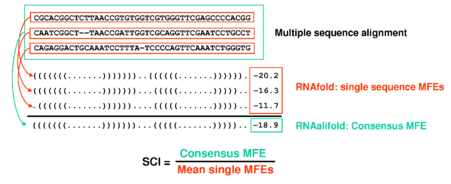
\includegraphics{Figs/sci.png}
\caption{pict}
\end{figure}

\begin{itemize}
\tightlist
\item
  The structure conservation index is an easy way to normalize an
  \texttt{RNAalifold} consensus MFE.
\end{itemize}

\textbf{z-score regression}\\
- The mean \(\mu\) and standard deviation \(\sigma\) of random samples
of a given sequence are functions of the length and the base
composition:
\[\mu,\sigma\left( {length,\frac{GC}{AT},\frac{G}{C},\frac{A}{T}} \right)\]
- It is therefore be possible to \emph{calculate} \(z\)-scores by
solving this 5 dimensional regression problem.

\textbf{SVM Classification}\\

\begin{figure}[htbp]
\centering
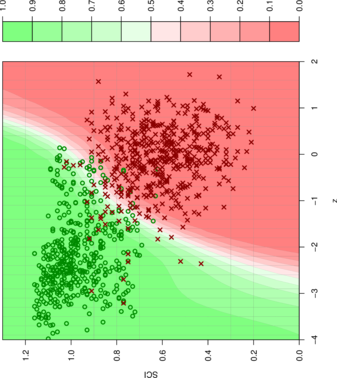
\includegraphics{Figs/contour.png}
\caption{pict}
\end{figure}

\begin{itemize}
\tightlist
\item
  A support vector machine learning algorithm is used to classify an
  alignment based on \(z\)-score and structure conservation index.
\end{itemize}

\textbf{Installation of RNAz}\\
Installation is done according to the instructions used by the
\texttt{ViennaRNA\ Package}. Just use the \texttt{-\/-prefix} option as
mentioned earlier and add the PATH to \texttt{.bashrc}

\begin{itemize}
\tightlist
\item
  RNAz is available at:
  \href{http://www.tbi.univie.ac.at/\%7Ewash/RNAz}{http://www.tbi.univie.ac.at/\textasciitilde{}wash/RNAz}
\item
  Package includes the core program \texttt{RNAz} in ISO \texttt{C}, a
  set of helper programs in Perl, and an extensive manual.
\end{itemize}

\textbf{Basic usage of RNAz}\\
 \hyperdef{}{textcolor2}{\label{textcolor2}}{* where to get examples
from (RNAz install package) - commands work with v2 but txt needs to be
adopted *} - \texttt{RNAz} reads one or more multiple sequence
alignments in \texttt{clustalw} or MAF format.

\begin{verbatim}
$ RNAz --help
$ RNAz tRNA.aln
$ RNAz --both-strands --predict-strand tRNA.maf
\end{verbatim}

\textbf{Advanced usage of RNAz}\\
- \texttt{RNAz} is limited to a maximum alignment length of 400 columns
and a maximum number of 6 sequences. To process larger alignments a set
of Perl helper scripts are used. - Selecting one or more subsets of
sequences from an alignment with more than 6 sequences:

\begin{verbatim}
$ rnazSelectSeqs.pl miRNA.maf |RNAz
$ rnazSelectSeqs.pl --num-seqs=4 --num-samples=3 miRNA.maf |RNAz
\end{verbatim}

\begin{itemize}
\tightlist
\item
  Scoring long alignments in overlapping windows:
\end{itemize}

\begin{verbatim}
$ rnazWindow.pl --window=120 --slide=40 unknown.aln \
              | RNAz --both-strands
\end{verbatim}

\subsubsection{Large scale screens}{Large scale screens}\label{large-scale-screens}

The \texttt{RNAz} package provides a set of Perl scripts that implement
a complete analysis pipeline suitable for medium to large scale screens
of genomic data.

\textbf{General procedure}\\
1. Obtain or create multiple sequence alignments in MAF format 2. Run
through the \texttt{RNAz} pipeline:

\begin{figure}[htbp]
\centering
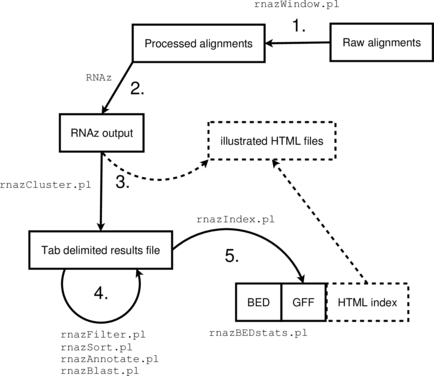
\includegraphics{Figs/flowchart.png}
\caption{pict}
\end{figure}

\textbf{Examples in this tutorial}\\
1. Align Epstein Barr Virus genome (Acc.no: NC\_007605) to two related
primate viruses (Acc.nos: NC\_004367, NC\_006146) using \texttt{multiz}
and run it through the \texttt{RNAz} pipeline.
\hyperdef{}{textcolor3}{\label{textcolor3}}{* where are this data
comeing from? file from NCBI differs from those hidden in
genefinding/rnaz/herpes *} 2. Analyze snoRNA cluster in the human genome
for conserved RNA structures: download pre-computed alignments from the
UCSC genome browser and run it through the \texttt{RNAz} pipeline

\textbf{Example a: Preparation of data}\\
- \texttt{multiz} and \texttt{blastz} are available here:
\url{http://www.bx.psu.edu/miller_lab/} - Download the viral genomes in
FASTA format and reformat the header strictly according to the rules
given in the \texttt{multiz} documentation
(\url{http://www.bx.psu.edu/miller_lab/dist/tba_howto.pdf}), e.g.: - You
have to edit the ''multiz '' \texttt{Makefile} and replace

\begin{verbatim}
<div id="verbatim-88" class="verbatim">

``` {.commands}
CFLAGS = -Wall -Wextra -Werror
```

</div>

with

<div id="verbatim-89" class="verbatim">

``` {.commands}
CFLAGS = -Wall -Wextra #-Werror
```

</div>

and then simply use the `make` command to compile both programs.
\end{verbatim}

\hyperdef{}{textcolor4}{\label{textcolor4}}{* dont understand what to do
*}

\hyperdef{}{verbatim-90}{\label{verbatim-90}}
\begin{verbatim}
>NC_007605:genome:1:+:149696
AGAATTCGTCTTGCTCTATTCACCCTTACTTTTCTTCTTGCCCGTTCTCTTTCTTAGTAT
GAATCCAGTATGCCTGCCTGTAATTGTTGCGCCCTACCTCTTTTGGCTGGCGGCTATTGC
CGCCTCGTGTTTCACGGCCTCAGTTAGTACCGTTGTGACCGCCACCGGCTTGGCCCTCTC
ACTTCTACTCTTGGCAGCAGTGGCCAGCTCATATGCCGCTGCACAAAGGAAACTGCTGAC
ACCGGTGACAGTGCTTACTGCGGTTGTCACTTGTGAGTACACACGCACCATTTACAATGC
ATGATGTTCGTGAGATTGATCTGTCTCTAACAGTTCACTTCCTCTGCTTTTCTCCTCAGT
CTTTGCAATTTGCCTAACATGGAGGATTGAGGACCCACCTTTTAATTCTCTTCTGTTTGC
[...]
\end{verbatim}

\textbf{Example a: Aligning viral genomes}\\
- To get a multiple alignment a phylogenetic tree and the following
three steps are necessary: 1. Run \texttt{blastz} each vs.~each 2.
Combine blastz results to multiple sequence alignments 3. Project raw
alignments to a reference sequence. - The corresponding commands:

\begin{verbatim}
all_bz - "((NC_007605 NC_006146) NC_004367)" | bash
tba "((NC_007605 NC_006146) NC_004367)" \
*.sing.maf raw-tba.maf
maf_project raw-tba.maf NC_007605 > final.maf
\end{verbatim}

\begin{itemize}
\tightlist
\item
  Note: The tree is given in NEWICK like format with blanks instead of
  commas. The sequence data files must be named exactly like the names in
  this tree and in the FASTA headers.
\end{itemize}

\textbf{Example a: Running the pipeline I}\\
- First the alignments are filtered and sliced in overlapping windows:

\begin{verbatim}
$ rnazWindow.pl < final.maf > windows.maf
\end{verbatim}

\begin{itemize}
\tightlist
\item
  \texttt{RNAz} is run on these windows:
\end{itemize}

\begin{verbatim}
$ RNAz --both-strands --show-gaps --cutoff=0.5 windows.maf \
       > rnaz.out
\end{verbatim}

\begin{itemize}
\tightlist
\item
  Overlapping hits are combined to ``loci'' and visualized on a
  web-site:
\end{itemize}

\begin{verbatim}
$ rnazCluster.pl --html rnaz.out > results.dat
\end{verbatim}

\textbf{Example a: Running the pipeline II}\\
- The predicted hits are compared with available annotation of the
genome:

\begin{verbatim}
$ rnazAnnotate.pl --bed annotation.bed results.dat \
         > results_annotated.dat
\end{verbatim}

\begin{itemize}
\tightlist
\item
  The results file is formatted in a HTML overview page:
\end{itemize}

\begin{verbatim}
$ rnazIndex.pl --html results_annotated.dat \
         > results/index.html
\end{verbatim}

\textbf{Example a: Statistics on the results}\\
- \texttt{rnazIndex.pl} can be used to generate a BED formatted
annotation file which can be analyzed using \texttt{rnazBEDstats.pl}
(after sorting, for the case the input alignments were unsorted)''

\begin{verbatim}
$ rnazIndex.pl --bed results.dat | \
         rnazBEDsort.pl | rnazBEDstats.pl
\end{verbatim}

\begin{itemize}
\tightlist
\item
  RNAzfilter.pl can be used to filter the results by different criteria. In
  this case it gives us all loci with P\$\textgreater{}\$0.9'':
\end{itemize}

\begin{verbatim}
$ rnazFilter.pl "P>0.9" results.dat | \
         rnazIndex.pl --bed | \
         rnazBEDsort.pl | rnazBEDstats.pl
\end{verbatim}

\begin{itemize}
\tightlist
\item
  To get an estimate on the (statistical) false positives one can repeat
  the complete screen with randomized alignments:
\end{itemize}

\begin{verbatim}
$ rnazRandomizeAln final.maf > random.maf
\end{verbatim}

\textbf{Example b: Obtaining pre-computed alignments from UCSC}\\
- Go to the UCSC genome browser
(\href{http://genome.ucsc.edu/}{http://genome.ucsc.edu}) and go to
``Tables''. Download ``multiz17'' alignments in MAF format for the
region: chr11:93103000-93108000

\begin{figure}[htbp]
\centering
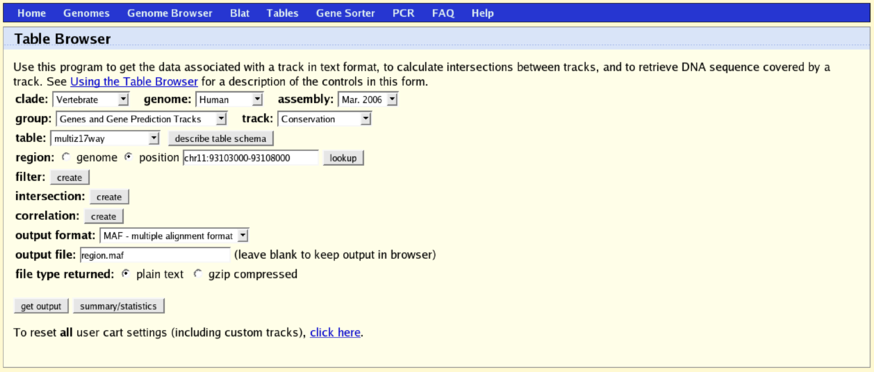
\includegraphics{Figs/table-browser.png}
\caption{pict}
\end{figure}

\textbf{Example b: Running the pipeline}\\
- The Perl scripts are run in the same order as in Example 1:

\begin{verbatim}
$ rnazWindow.pl --min-seqs=4 region.maf > windows.maf
$ RNAz --both-strands --show-gaps --cutoff=0.5 windows.maf \
         > rnaz.out
$ rnazCluster.pl --html rnaz.out > results.dat
$ rnazAnnotate.pl --bed annotation.bed results.dat \
         > results_annotated.dat
$ rnazIndex.pl --html results_annotated.dat \
         > results/index.html
\end{verbatim}

\begin{itemize}
\tightlist
\item
  The results can be exported as UCSC BED file which can be displayed in
  the genome browser:
\end{itemize}

\begin{verbatim}
$ rnazIndex.pl --bed --ucsc results.dat > prediction.bed
\end{verbatim}

\textbf{Example b: Visualizing the results on the genome browser}\\
- Upload the BED file as ``Custom Track''\ldots{}

\begin{figure}[htbp]
\centering
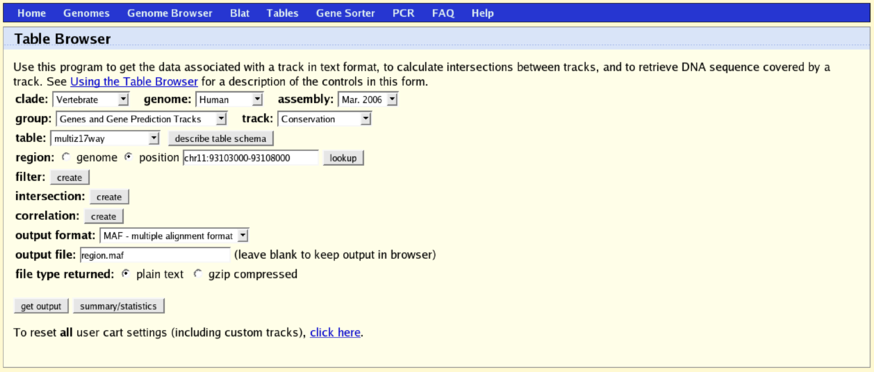
\includegraphics{Figs/table-browser.png}
\caption{pict}
\end{figure}

\begin{itemize}
\tightlist
\item
  \ldots{}and have a look at the results:
\end{itemize}

\begin{figure}[htbp]
\centering

\includegraphics{Figs/snos.png}
\caption{pict}
\end{figure}

\textbackslash{}let \textbackslash{}prOteCt \textbackslash{}relax
\textbackslash{}Protect \textbackslash{}gl:nopartrue

\hyperdef{}{sidebar}{\label{sidebar}}
\begin{itemize}
\tightlist
\item
  \hyperref[sec1]{RNA Web Services{}}

  \begin{itemize}
  \tightlist
  \item
    \hyperref[sec1]{Useful Web Services}
  \end{itemize}
\item
  \hyperref[sec2]{Get started{}}

  \begin{itemize}
  \tightlist
  \item
    \hyperref[sec2ux5f1]{Typographical Conventions}
  \item
    \hyperref[sec2ux5f2]{Data Files}
  \item
    \hyperref[sec2ux5f3]{Terminal, Command line and Editor}
  \item
    \hyperref[sec2ux5f4]{Installing Software from Source}
  \item
    \hyperref[sec2ux5f5]{Build the \texttt{ViennaRNA\ Package}}
  \item
    \hyperref[sec2ux5f6]{What's in the \texttt{ViennaRNA\ Package}}
  \item
    \hyperref[sec2ux5f7]{The Input File Format}
  \end{itemize}
\item
  \hyperref[sec3]{Structure Prediction on single Sequences{}}

  \begin{itemize}
  \tightlist
  \item
    \hyperref[sec3ux5f1]{The Program \texttt{RNAfold}}
  \item
    \hyperref[sec3ux5f2]{The Program \texttt{RNApvmin}}
  \item
    \hyperref[sec3ux5f3]{The Program \texttt{RNAsubopt}}
  \end{itemize}
\item
  \hyperref[sec4]{RNA folding kinetics{}}

  \begin{itemize}
  \tightlist
  \item
    \hyperref[sec4ux5f1]{RNA2Dfold}
  \item
    \hyperref[sec4ux5f2]{barriers \& treekin}
  \end{itemize}
\item
  \hyperref[sec5]{Sequence Design{}}

  \begin{itemize}
  \tightlist
  \item
    \hyperref[sec5ux5f1]{The Program \texttt{RNAinverse}}
  \item
    \hyperref[sec5ux5f2]{switch.pl}
  \end{itemize}
\item
  \hyperref[sec6]{RNA-RNA Interactions{}}

  \begin{itemize}
  \tightlist
  \item
    \hyperref[sec6ux5f1]{The Program \texttt{RNAcofold}}
  \item
    \hyperref[sec6ux5f2]{Concentration Dependency}
  \item
    \hyperref[sec6ux5f3]{Finding potential binding sites with RNAduplex}
  \end{itemize}
\item
  \hyperref[sec7]{Consensus Structure Prediction{}}

  \begin{itemize}
  \tightlist
  \item
    \hyperref[sec7ux5f1]{The Program \texttt{RNAalifold}}
  \end{itemize}
\item
  \hyperref[sec8]{Structural Alignments{}}

  \begin{itemize}
  \tightlist
  \item
    \hyperref[sec8ux5f1]{Manually correcting Alignments}
  \item
    \hyperref[sec8ux5f2]{Automatic structural alignments}
  \end{itemize}
\item
  \hyperref[sec9]{Noncoding RNA gene prediction{}}

  \begin{itemize}
  \tightlist
  \item
    \hyperref[sec9ux5f1]{QRNA}
  \item
    \hyperref[sec9ux5f2]{AlifoldZ}
  \item
    \hyperref[sec9ux5f3]{RNAz}
  \item
    \hyperref[sec9ux5f4]{Large scale screens}
  \end{itemize}
\end{itemize}

\hyperref[]{Top}

\href{https://www.tbi.univie.ac.at/legal.html}{Legal Details}

\end{document}
